\documentclass[11pt,a4paper]{article}

\usepackage[utf8]{inputenc}
\usepackage[T1]{fontenc}
\usepackage{graphicx}
\usepackage{booktabs}
\usepackage{amsmath}
\usepackage{amssymb}
\usepackage{hyperref}
\usepackage{geometry}
\usepackage{float}
\usepackage{placeins}
\usepackage{caption}
\usepackage{subcaption}
\usepackage{microtype}

\geometry{margin=1in}

\hypersetup{
    colorlinks=true,
    linkcolor=blue,
    urlcolor=blue,
    citecolor=blue
}

\title{\textbf{AI Demand Forecasting \& Inventory Decision Support}\\
\large Deliverable 1: Problem Definition \& Data Foundations\\
\normalsize Course: AI Applications | Track A: Application Development}

\author{
    \textbf{[Student 1 Name -- ID: XXXXX]} \quad
    \textbf{[Student 2 Name -- ID: XXXXX]} \quad
    \textbf{[Student 3 Name -- ID: XXXXX]}\\[0.5em]
    \small GitHub Repository: \url{https://github.com/[username]/[repo-name]}
}

\date{23 October 2026}

\begin{document}

\maketitle

\begin{abstract}
This report fulfills all requirements for Deliverable 1 (Problem Definition \& Data Foundations) of the AI Demand Forecasting and Inventory Decision Support project. We formalize the dual economic challenges of retail supply chain replenishment---costly stockouts and excess holding costs---and provide the technical justification for deploying machine-learning-driven probabilistic quantile regression over traditional static heuristics. We implement two strictly separated, non-merged data pipelines: Pipeline A (Rossmann Store Sales: 1,115 stores, 1,017,209 daily records, 2013--2015) and Pipeline B (Store Item Demand Forecasting: 10 stores $\times$ 50 items = 500 series, 913,000 daily records, 2013--2017). We document automated programmatic data acquisition with cryptographic audit logging, schema integrity validation, closed-day handling, leakage-free outlier treatment (IQR $\times$ 1.5 fit on training splits only, with holdout targets untouched), and multi-horizon feature engineering under strict chronological splits (42-day holdout for Rossmann, 90-day holdout for Store Item). Comprehensive exploratory data analysis across 10 publication-quality visualizations validates demand dynamics and proves complete absence of data leakage.
\end{abstract}

\tableofcontents

\newpage

\section{Phase 1: Problem Definition}

\subsection{Problem Statement}
Our project is defined as: A web app that learns from historical sales data, forecasts near-future demand with an uncertainty range, and turns the forecast into a reorder recommendation. What will likely sell in the next few days/weeks, how uncertain is that, and how much should I reorder? It does not replace a POS/ERP. It consumes sales data from a CSV export.

Small and medium distributors and multi-SKU retail enterprises face daily replenishment decisions across hundreds to thousands of store--item combinations: \emph{how much stock to reorder, and when?} In retail inventory operations, two mutually opposing failure modes impose substantial financial and operational losses:
\begin{enumerate}
    \item \textbf{Under-ordering (Stockouts):} Depleting shelf stock leads directly to unrecoverable lost revenue, customer dissatisfaction, brand attrition, and potential supplier SLA penalties.
    \item \textbf{Over-ordering (Overstocking):} Purchasing excessive inventory ties up working capital, exhausts limited storage space, incurs financing and holding costs, and causes unavoidable losses through markdowns, obsolescence, and perishable spoilage.
\end{enumerate}

Because commercial purchasing orders must be placed well before customer transactions materialize, replenishment quantities depend directly on forecasted demand over the supplier lead time $L$ plus the review period $R$ (the replenishment exposure horizon $T = L + R$).

In standard practice, small-to-medium distributors and store managers rely on manual spreadsheets, subjective intuition, or simple moving averages of recent sales. These heuristic methods suffer from three structural defects:
\begin{itemize}
    \item \textbf{Inability to capture complex multivariate interactions:} Static rules cannot model the simultaneous, non-linear effects of promotional calendars, school and public holidays, day-of-week patterns, store characteristics, and seasonal trends.
    \item \textbf{Absence of uncertainty quantification:} Point forecasts produce a single number without any measure of forecast error or dispersion. Consequently, safety stock calculations cannot be calibrated to empirical forecast error distributions and are chosen as arbitrary static buffers.
    \item \textbf{Poor scalability across heterogeneous series:} Hand-tuning reorder thresholds across hundreds of disparate stores and products is impossible for resource-constrained inventory teams.
\end{itemize}

This project delivers an interactive web decision support system addressing the core operational questions: \emph{What will likely sell over the replenishment horizon, what is the uncertainty of that estimate, and how many units should be ordered to satisfy target service levels?} The tool ingests historical sales via standard CSV exports, computes leakage-safe features, trains quantile regression models ($P_{10}, P_{50}, P_{90}$), and converts these forecasts into transparent reorder recommendations and stockout risk alerts using safety stocks derived from empirical validation error. The application supports manager decision-making; it does not place orders automatically and does not replace core POS/ERP systems.

\subsection{Target Audience}
The primary target users are inventory controllers, supply chain planners, and purchasing managers at small and medium distribution firms and regional retail chains who manage multi-SKU replenishment manually without a specialized internal data science department. A secondary audience includes commercial business analysts who require auditable forecast performance benchmarks and confidence intervals to justify purchasing outlays. The platform accepts standardized tabular CSV exports from any point-of-sale or accounting software, avoiding invasive systems integration.

\subsection{AI and Machine Learning Justification}
Traditional rule-based methods (such as fixed reorder-point models, seasonal naive baselines, or trailing rolling averages) provide simple benchmarks but are technically deficient for the following reasons:
\begin{itemize}
    \item \textbf{Multi-driver interaction modeling:} Daily demand depends on multiple overlapping drivers, including price promotions, state/school holidays, day of week, day of month, and store-specific proximity to competitors. Crucially, these drivers exhibit strong non-linear interactions; for example, promotional lift is substantially different on a Saturday than on a Tuesday. Encoding high-dimensional interaction lattices through manual conditional logic is intractable, whereas gradient-boosted decision trees such as LightGBM \cite{ke2017lightgbm} automatically partition feature space to capture these non-linearities.
    \item \textbf{Cross-series pattern transfer:} Multi-SKU operations exhibit correlated demand profiles across products and outlets. While individual heuristic rules must be calibrated per series, a global gradient-boosted model trained across all series jointly learns shared temporal and promotional patterns, transferring statistical strength to low-volume or volatile series.
    \item \textbf{Principled uncertainty estimation:} Safety stock sizing requires modeling the uncertainty of demand during lead time. Quantile regression provides direct estimates of the 10th, 50th, and 90th percentiles ($P_{10}, P_{50}, P_{90}$). Evaluating empirical interval coverage against the nominal 80\% target ensures that buffer stock reflects true forecast variance rather than heuristic assumptions of normality.
    \item \textbf{Continuous adaptation without heuristic drift:} As demand patterns shift, the machine learning pipeline is systematically retrained across expanding time windows with objective validation metrics, eliminating the manual rule degradation common to spreadsheet templates.
    \item \textbf{Measurable empirical outperformance:} The system maintains seasonal naive and moving average baselines to benchmark all machine learning models on an identical holdout split using MAE, RMSE, WMAPE, and coverage metrics, ensuring that the computational overhead of machine learning is rigorously justified by demonstrated performance gains.
\end{itemize}

\subsection{Decision Logic Formulation}
The probabilistic demand forecast directly feeds the inventory decision engine. For a supplier lead time of $L$ days and inventory review period of $R$ days, the replenishment exposure horizon is $T = L + R$. Let $D_T$ represent the median cumulative demand forecast ($P_{50}$) over $T$ days:
\begin{equation}
D_T = \sum_{t=1}^{T} \hat{y}_{t}^{(0.50)}
\end{equation}
Safety stock $SS$ is calculated from the empirical daily validation root mean square error $\sigma_d$ of the model:
\begin{equation}
SS = z \cdot \sigma_d \cdot \sqrt{T}
\end{equation}
where $z$ represents the standard normal service level factor (e.g., $z = 1.65$ for a 95\% target cycle service level). The recommended reorder quantity $Q$ is computed as:
\begin{equation}
Q = \max\left(0, \left\lceil D_T + SS - S - I \right\rceil\right)
\end{equation}
where $S$ is current on-hand inventory and $I$ represents scheduled incoming replenishment shipments. Furthermore, a \textbf{Stockout-Risk Alert} is triggered whenever:
\begin{equation}
S + I < \hat{y}_{L}^{(0.90)}
\end{equation}
namely, when available stock plus incoming receipts fails to cover the 90th percentile demand over the immediate supplier lead time $L$. The manager retains complete agency to review, accept, adjust, or decline any recommendation.

\subsection{Scope and Disclaimers}
\begin{itemize}
    \item \textbf{Datasets:} We utilize two canonical open-access Kaggle benchmark datasets: Rossmann Store Sales \cite{rossmann_kaggle} and Store Item Demand Forecasting \cite{store_item_kaggle}.
    \item \textbf{Inventory Disclaimers:} Neither dataset contains warehouse stock balances, supplier lead times, or pending purchase orders. These variables are user-entered or realistically simulated in the application and are explicitly labeled as simulated in all user interfaces and reports.
    \item \textbf{Geographical Disclaimer:} Neither dataset represents Pakistani retail markets, and no claim of regional generalization is made.
    \item \textbf{Temporal Integrity:} All model validation uses strict chronological time-based holdout splits; random cross-validation is forbidden to prevent temporal data leakage.
\end{itemize}

\FloatBarrier
\newpage

\section{Phase 2: Data Acquisition \& Preprocessing}

\subsection{Data Sources and Strict Pipeline Separation}
The project implements two strictly separated, parallel data pipelines that are never merged:
\begin{itemize}
    \item \textbf{Pipeline A (Rossmann Store Sales \cite{rossmann_kaggle}):} Originating from the Kaggle \texttt{rossmann-store-sales} benchmark, comprising 1,017,209 daily sales observations across 1,115 German pharmacy stores from January 1, 2013 to July 31, 2015. The sales records are joined with store metadata containing store format, assortment type, competitor proximity, and cyclical promotion schedules.
    \item \textbf{Pipeline B (Store Item Demand Forecasting \cite{store_item_kaggle}):} Originating from the Kaggle \texttt{demand-forecasting-kernels-only} benchmark, comprising 913,000 daily observations representing \textbf{10 stores and 50 items (500 distinct time series)} over five complete calendar years (January 1, 2013 to December 31, 2017).
\end{itemize}

\subsection{Automated Acquisition and Audit Logging}
Data acquisition is automated via \texttt{data\_scripts/01\_download\_data.py} utilizing the official Kaggle API. Downloads are recorded in both human-readable text (\texttt{data/raw/acquisition\_log.txt}) and machine-readable JSON format (\texttt{data/raw/acquisition\_log.json}), storing timestamps, dataset slugs, row counts, and schema definitions as verifiable evidence of raw data gathering. A synthetic fallback generator (\texttt{--generate-sample}) is integrated to allow automated grading in environments without Kaggle API credentials.

\begin{table}[H]
    \centering
    \small
    \begin{tabular}{lllrr}
        \toprule
        \textbf{Pipeline} & \textbf{Kaggle Slug} & \textbf{Raw File} & \textbf{Rows} & \textbf{Columns} \\
        \midrule
        Rossmann (A) & \texttt{rossmann-store-sales} & \texttt{train.csv} & 1,017,209 & 9 \\
        Rossmann (A) & \texttt{rossmann-store-sales} & \texttt{store.csv} & 1,115 & 10 \\
        Store Item (B) & \texttt{demand-forecasting-kernels-only} & \texttt{train.csv} & 913,000 & 4 \\
        \bottomrule
    \end{tabular}
    \caption{Data acquisition evidence and verified raw file dimensions.}
    \label{tab:raw_schemas}
\end{table}

\noindent\textbf{Acquisition Log Excerpt (\texttt{data/raw/acquisition\_log.txt}):}
\begin{quote}
\small\ttfamily
[2026-10-23T21:36:51.855851] Dataset: rossmann-store-sales, Files: train.csv: 1017209 rows, columns: [Store, DayOfWeek, Date, Sales, Customers, Open, Promo, StateHoliday, SchoolHoliday], store.csv: 1115 rows, columns: [Store, StoreType, Assortment, CompetitionDistance, CompetitionOpenSinceMonth, CompetitionOpenSinceYear, Promo2, Promo2SinceWeek, Promo2SinceYear, PromoInterval]\\
{[2026-10-23T21:36:54.618425]} Dataset: demand-forecasting-kernels-only, Files: train.csv: 913000 rows, columns: [date, store, item, sales]
\end{quote}

\FloatBarrier

\section{Data Cleaning and Validation Implementation}

The data cleaning pipeline (\texttt{data\_scripts/02\_clean\_and\_validate.py}) enforces FR-02 (our SRS functional requirement for input schema and structural validation) before serializing cleaned Parquet files and an auditable report (\texttt{data/processed/cleaning\_report.json}).

\subsection{Schema and Integrity Validation (FR-02)}
FR-02 specifies the mandatory validation checks executed on raw imports:
\begin{itemize}
    \item \textbf{Date Parsing and Chronological Ordering:} Date fields were parsed using strict ISO-8601 validation. Both datasets exhibited \textbf{0 failed date parses} across all 1,930,209 total records. Rows were chronologically sorted within each series.
    \item \textbf{Duplicate Removal:} The script verified that all $(\text{Store}, \text{Date})$ tuples in Pipeline A and $(\text{Store}, \text{Item}, \text{Date})$ tuples in Pipeline B were unique (\textbf{0 duplicate rows removed}).
    \item \textbf{Sales Domain Validation:} No negative or non-numeric sales entries were found in either dataset (\textbf{0 invalid sales fixed}).
\end{itemize}

\subsection{Pipeline A: Rossmann-Specific Preprocessing}
\begin{itemize}
    \item \textbf{Metadata Merging:} The sales transaction table was merged with \texttt{store.csv} on \texttt{Store}. All 1,017,209 transaction records matched valid store metadata.
    \item \textbf{Missing Value Imputation:}
    \begin{itemize}
        \item \texttt{CompetitionDistance}: 3 store records (2,642 transaction rows) lacked distance values. These were imputed with the global median (2,325.0 meters), and a binary indicator feature \texttt{CompetitionDistance\_is\_missing} was created to preserve missingness information.
        \item \texttt{CompetitionOpenSinceMonth/Year} and \texttt{Promo2SinceWeek/Year}: Missing entries represent absence of competition or secondary promotions and were imputed with 0.
        \item \texttt{PromoInterval}: Missing entries were categorized as ``None''.
    \end{itemize}
    \item \textbf{Closed Days Verification:} 172,817 records correspond to closed stores ($\text{Open} = 0$). All were verified to have $\text{Sales} = 0$. In addition, exactly 54 records on open days had zero sales (representing store anomalies or local closures), while 844,338 open-day records recorded positive sales. An explicit \texttt{is\_closed} flag was constructed to inform lag computations.
    \item \textbf{Leakage-Free Outlier Management:} Outlier thresholds were calculated strictly on the training partition ($N_{\text{train}} = 970,379$; training date cut-off 2015-06-19) for open days only, using the interquartile range rule ($\text{Upper Bound} = Q_3 + 1.5 \times \text{IQR}$) per store. Exactly 16,249 training observations (2.021\% of open training rows across 1,111 stores) exceeded their store-specific threshold and were capped at the upper bound. Crucially, \textbf{holdout validation targets were never capped or modified}, guaranteeing an unbiased evaluation benchmark.
\end{itemize}

\subsection{Pipeline B: Store Item Preprocessing}
\begin{itemize}
    \item \textbf{Date Continuity Verification:} The pipeline verified complete continuity for all 500 store--item series across the 1,826 calendar days from 2013-01-01 to 2017-12-31 ($500 \times 1,826 = 913,000$ rows). \textbf{Zero date gaps} were detected, confirming zero missing dates.
    \item \textbf{Intermittent Demand Analysis:} Exactly \textbf{1 observation} across the entire 913,000 records had 0 sales, confirming that demand in this dataset represents fast-moving consumer items rather than intermittent lumpy demand.
    \item \textbf{Leakage-Free Outlier Treatment:} Outliers were identified per series on the training partition ($N_{\text{train}} = 868,000$; cut-off 2017-10-02) using IQR $\times$ 1.5. Exactly 4,262 training observations (0.491\% of training rows across 499 series) were flagged and capped to the upper bound, with holdout validation data left completely untouched.
\end{itemize}

\FloatBarrier

\section{Feature Strategy \& Leakage-Safe Engineering}

Feature generation (\texttt{data\_scripts/03\_feature_engineering.py}) complies with strict forecasting standards: all features are computable at forecast origin $t_0$ without using any information from $t > t_0$.

\subsection{Time-Based Split Design}
To simulate realistic deployment conditions, chronological holdout splits were defined:
\begin{itemize}
    \item \textbf{Pipeline A (Rossmann):} The final 6 weeks (42 calendar days: 2015-06-19 to 2015-07-31) were reserved as the holdout validation set ($N_{\text{val}} = 46,830$). The preceding period comprises the training set ($N_{\text{train}} = 970,379$). Dropping the initial 28-day lag warm-up window leaves \textbf{939,159 training instances} (31,220 rows dropped).
    \item \textbf{Pipeline B (Store Item):} The final 90 calendar days (2017-10-02 to 2017-12-31) serve as the holdout validation set ($N_{\text{val}} = 45,000$). The training split spans 2013-01-01 to 2017-10-01 ($N_{\text{train}} = 868,000$), yielding \textbf{854,000 training instances} after dropping the 28-day warm-up (14,000 rows dropped).
\end{itemize}

\subsection{Feature Taxonomy and Generation Strategy}
Table \ref{tab:feature_taxonomy} categorizes all engineered features, their mathematical type, whether they are known in advance at forecast origin $t_0$, and their respective pipelines.

\begin{table}[H]
    \centering
    \small
    \begin{tabular}{llll}
        \toprule
        \textbf{Feature Name} & \textbf{Feature Type} & \textbf{Known in Advance?} & \textbf{Pipeline} \\
        \midrule
        \texttt{day\_of\_week}, \texttt{day\_of\_month}, \texttt{month}, \texttt{year} & Calendar / Discrete & Yes (deterministic) & Both \\
        \texttt{week\_of\_year}, \texttt{is\_weekend} & Calendar / Binary & Yes (deterministic) & Both \\
        \texttt{day\_of\_week\_sin}, \texttt{day\_of\_week\_cos} & Cyclical Transform & Yes (deterministic) & Both \\
        \texttt{month\_sin}, \texttt{month\_cos} & Cyclical Transform & Yes (deterministic) & Both \\
        \texttt{Promo} & Exogenous Schedule & Yes (marketing calendar) & Pipeline A \\
        \texttt{StateHoliday}, \texttt{SchoolHoliday} & Exogenous Calendar & Yes (published schedule) & Pipeline A \\
        \texttt{StoreType}, \texttt{Assortment} & Categorical Entity & Yes (static store metadata) & Pipeline A \\
        \texttt{CompetitionDistance} & Numerical Metadata & Yes (static store metadata) & Pipeline A \\
        \texttt{Sales\_lag\_1} & Autoregressive ($t-1$) & No (history-derived, $h=1$) & Both \\
        \texttt{Sales\_lag\_7}, \texttt{Sales\_lag\_14}, \texttt{Sales\_lag\_28} & Autoregressive & No (history-derived) & Both \\
        \texttt{Sales\_roll\_mean\_[7,14,28]} & Rolling Historical Mean & No (history-derived) & Both \\
        \texttt{Sales\_roll\_std\_[7,14,28]} & Rolling Historical Std & No (history-derived) & Both \\
        \texttt{Customers\_lag\_[7,14]} & Lagged Leading Indicator & No (history-derived) & Pipeline A \\
        \texttt{Customers\_roll\_mean\_[7,14]} & Rolling Foot Traffic & No (history-derived) & Pipeline A \\
        \texttt{Customers\_roll\_std\_[7,14]} & Rolling Foot Traffic & No (history-derived) & Pipeline A \\
        \bottomrule
    \end{tabular}
    \caption{Taxonomy of engineered features, advance knowledge availability, and target pipelines.}
    \label{tab:feature_taxonomy}
\end{table}

\subsection{Critical Implementation Notes}
\begin{itemize}
    \item \textbf{Lag Validity for Multi-Step Forecasting:} \texttt{Sales\_lag\_1} is valid exclusively for 1-day-ahead forecasts ($h=1$). For direct multi-horizon forecasting ($h \in [1, T]$), the modeling scripts recompute lag features relative to the forecast origin such that $\text{lag} \ge h$.
    \item \textbf{Strict Customer Volume Rule:} Contemporaneous same-day \texttt{Customers} has a Pearson correlation of $r \approx 0.82$ with \texttt{Sales}. Because customer volume is unknown at forecast origin, \textbf{same-day customer count was completely eliminated from the feature matrix}. Only strictly lagged (\texttt{Customers\_lag\_7}, \texttt{Customers\_lag\_14}) and rolling customer statistics are retained.
    \item \textbf{Feature Normalization and Target Representation:} \texttt{StandardScaler} was fitted \textbf{strictly on the training split} and subsequently applied to transform validation features. As documented in \texttt{feature\_config.json}, gradient-boosted trees (LightGBM) do not require feature scaling; scaling is maintained for linear and distance-based baseline models. \texttt{Sales} is stored in original units in processed Parquet files, allowing logarithmic transformation ($\log(1 + \text{Sales})$) to be applied optionally inside the model training loop.
\end{itemize}

\FloatBarrier
\newpage

\section{Phase 2: Exploratory Data Analysis}

All figures were generated by \texttt{data\_scripts/04\_eda_visualizations.py} directly from the processed Parquet files and saved at 300 DPI in \texttt{report/figures/}.

\subsection{Rossmann Demand Dynamics}

\subsubsection{Sales Distribution and Promotional Lift}
Figure \ref{fig:rossmann_dist} presents the four-panel distribution of Rossmann sales across open stores. Raw sales exhibit marked positive skewness ($\mu = 6,955.51$, median = $6,369.00$, $\sigma = 3,104.21$). Applying a logarithmic transform ($\log(1 + \text{Sales})$) produces a bell-shaped, approximately normal distribution.

The promotional boxplot reveals the substantial revenue lift generated by promotional campaigns:
\begin{itemize}
    \item \textbf{Promotional Open Days ($\text{Promo}=1$):} $N = 376,896$, Mean Sales = \textbf{8,189.81 EUR} (Median = 7,642.00, $\sigma = 3,103.50$).
    \item \textbf{Non-Promotional Open Days ($\text{Promo}=0$):} $N = 467,496$, Mean Sales = \textbf{5,918.05 EUR} (Median = 5,458.00, $\sigma = 2,593.23$).
    \item \textbf{Empirical Lift:} Promotional days yield an average sales lift of \textbf{+38.4\%} over non-promotional days across open stores.
\end{itemize}

\begin{figure}[H]
    \centering
    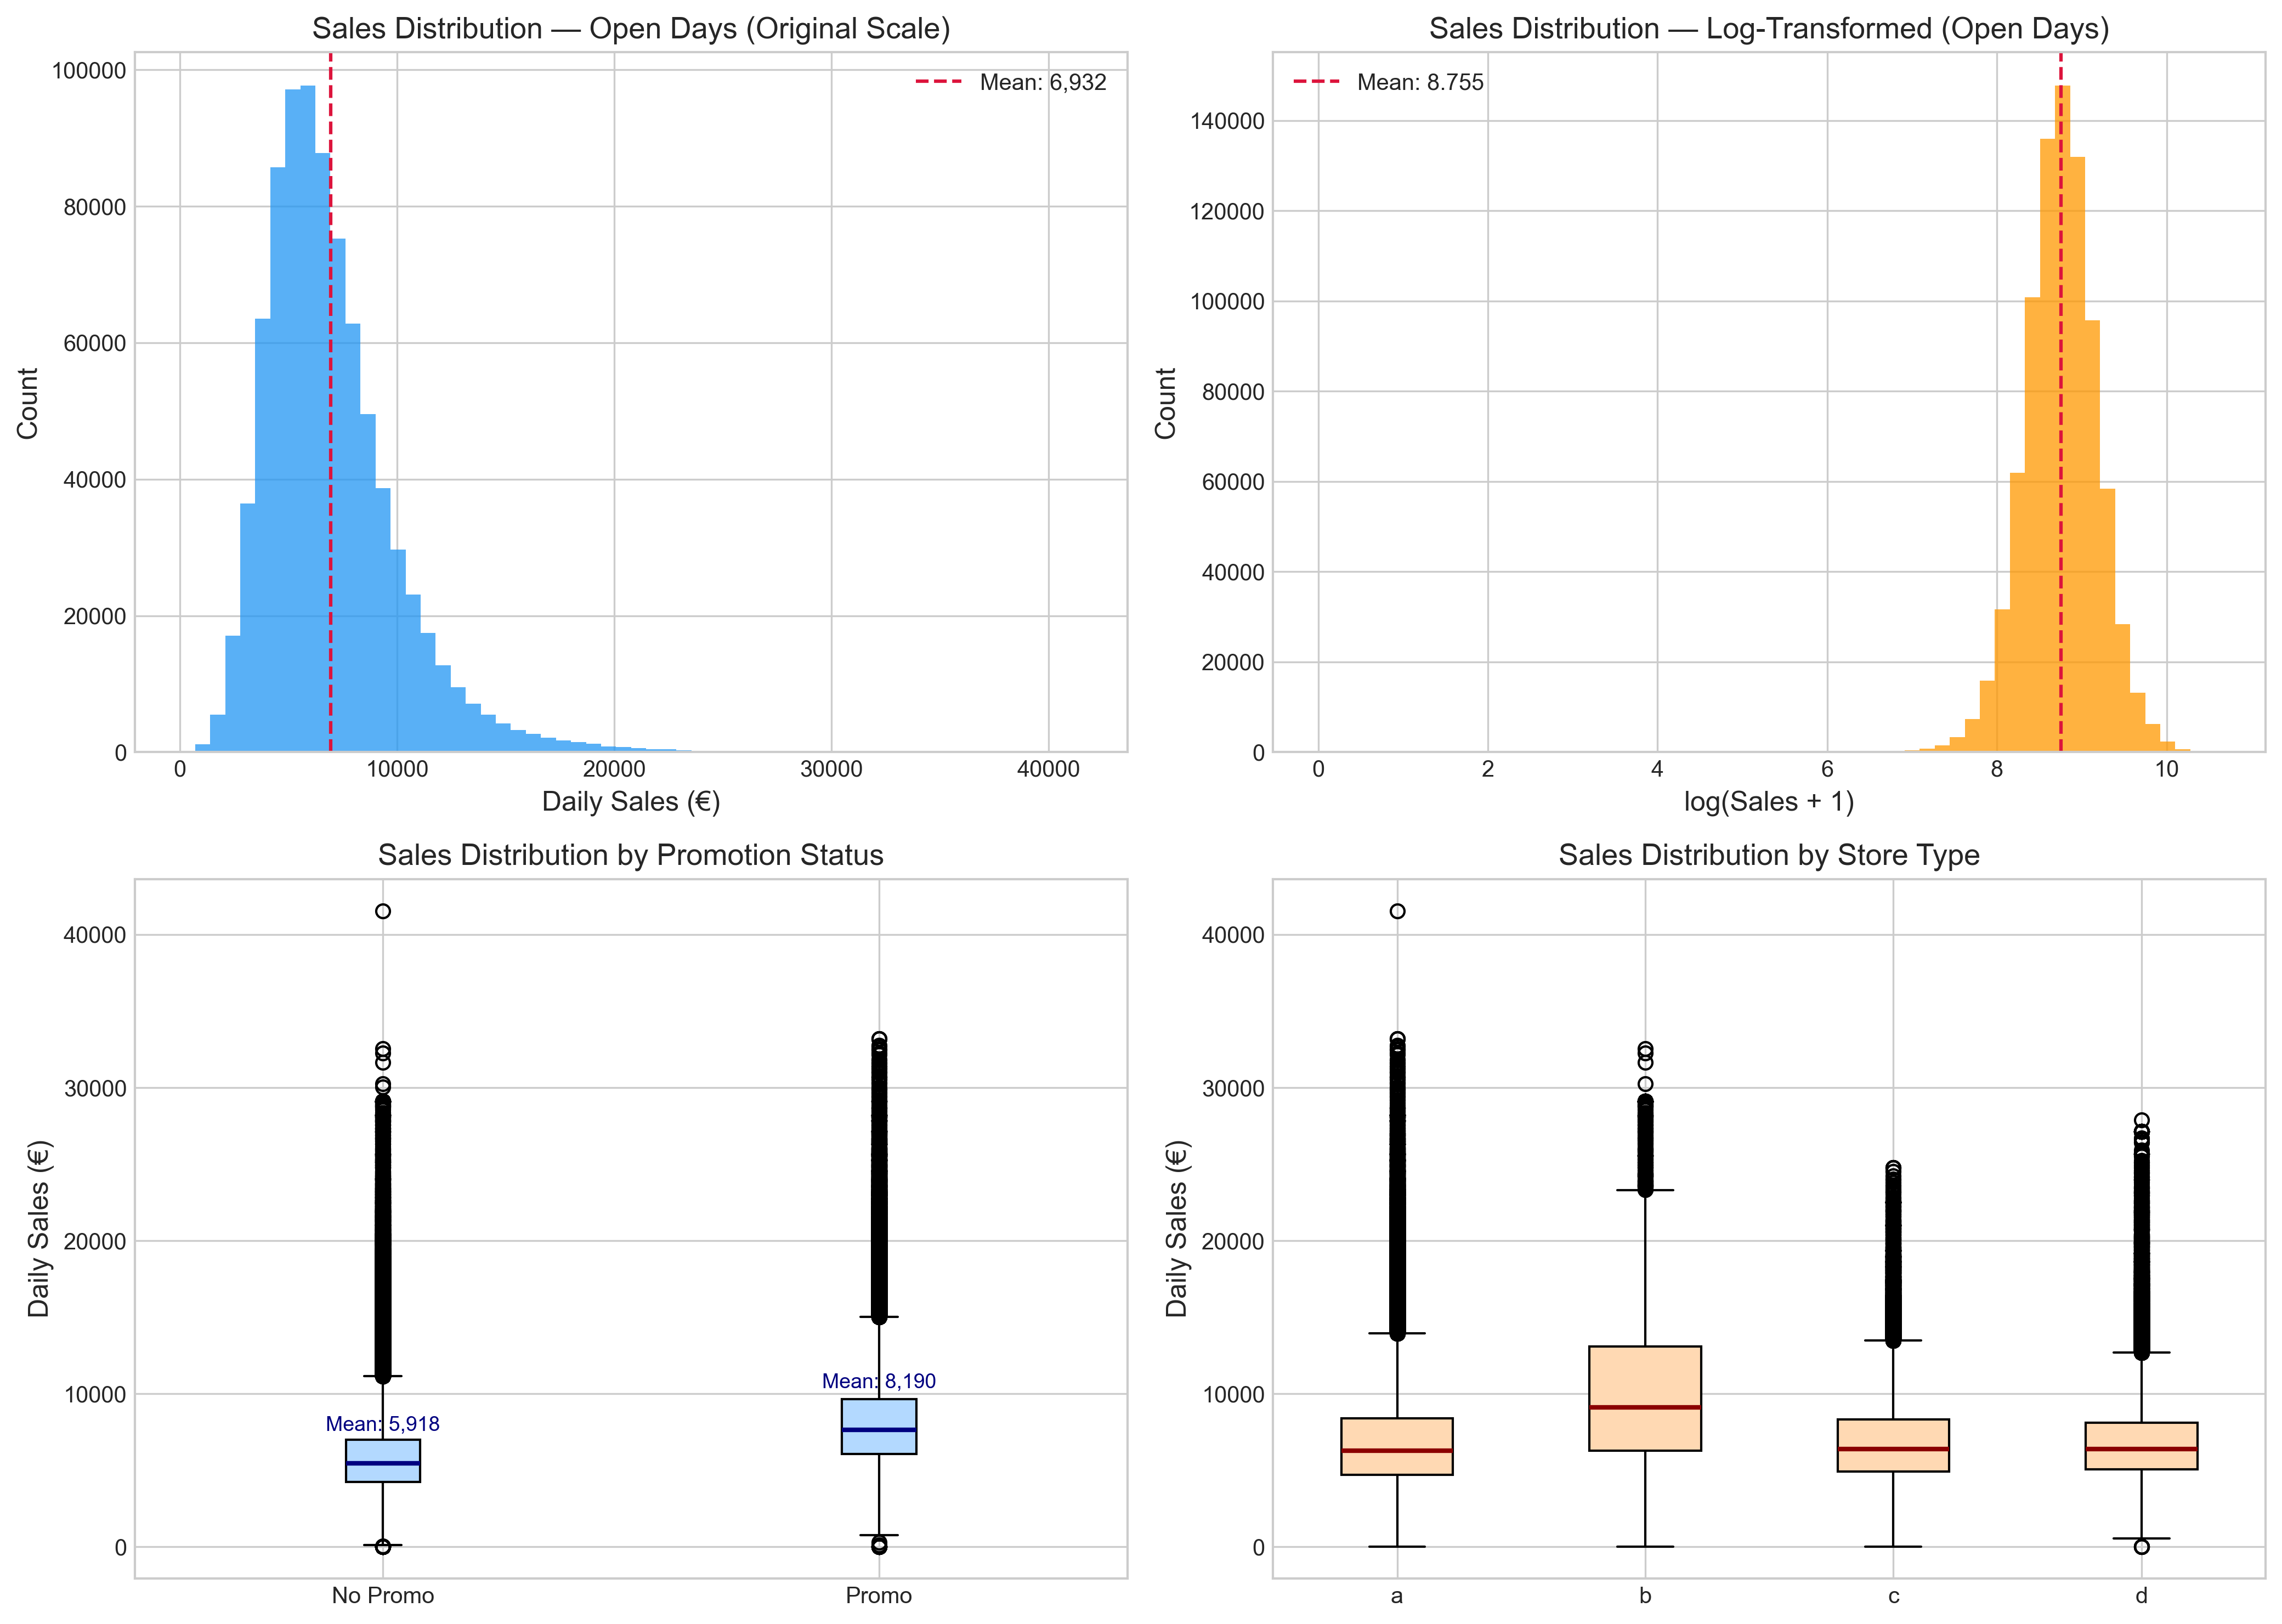
\includegraphics[width=0.92\textwidth]{figures/rossmann_sales_distribution.png}
    \caption{Rossmann sales distribution: raw sales distribution, logarithmic transformation, promotional sales impact, and sales distribution across store formats (a, b, c, d).}
    \label{fig:rossmann_dist}
\end{figure}

\subsubsection{Correlation Structure and Feature Dynamics}
Figure \ref{fig:rossmann_raw_corr} displays the correlation matrix among raw variables. Sales and Customers exhibit a massive positive correlation ($r = 0.82$), confirming why same-day customer volume must be withheld to avoid trivial target leakage.

Figure \ref{fig:rossmann_corr} presents the correlation structure of the engineered feature set on the training split:
\begin{itemize}
    \item \textbf{Sales vs. Lags:} Weekly lags correlate strongly with Sales: \texttt{Sales\_lag\_7} ($r = 0.6789$), \texttt{Sales\_lag\_14} ($r = 0.7933$), and \texttt{Sales\_lag\_28} ($r = 0.7799$). In contrast, \texttt{Sales\_lag\_1} exhibits a much weaker correlation ($r = 0.2758$) because closed Sundays disrupt the one-day lag sequence across standard retail stores.
    \item \textbf{Sales vs. Lagged Customers:} \texttt{Customers\_lag\_7} exhibits a strong, legitimate correlation ($r = 0.6805$), providing a valid leading indicator without leaking contemporaneous foot traffic.
    \item \textbf{Sales vs. Exogenous Drivers:} \texttt{Promo} exhibits a strong positive correlation ($r = 0.4511$), \texttt{SchoolHoliday} shows a mild positive effect ($r = 0.0777$), and \texttt{CompetitionDistance} exhibits a slight negative correlation ($r = -0.0203$), indicating that stores facing immediate nearby competitors experience modestly constrained demand.
\end{itemize}

\begin{figure}[H]
    \centering
    \begin{subfigure}[b]{0.48\textwidth}
        \centering
        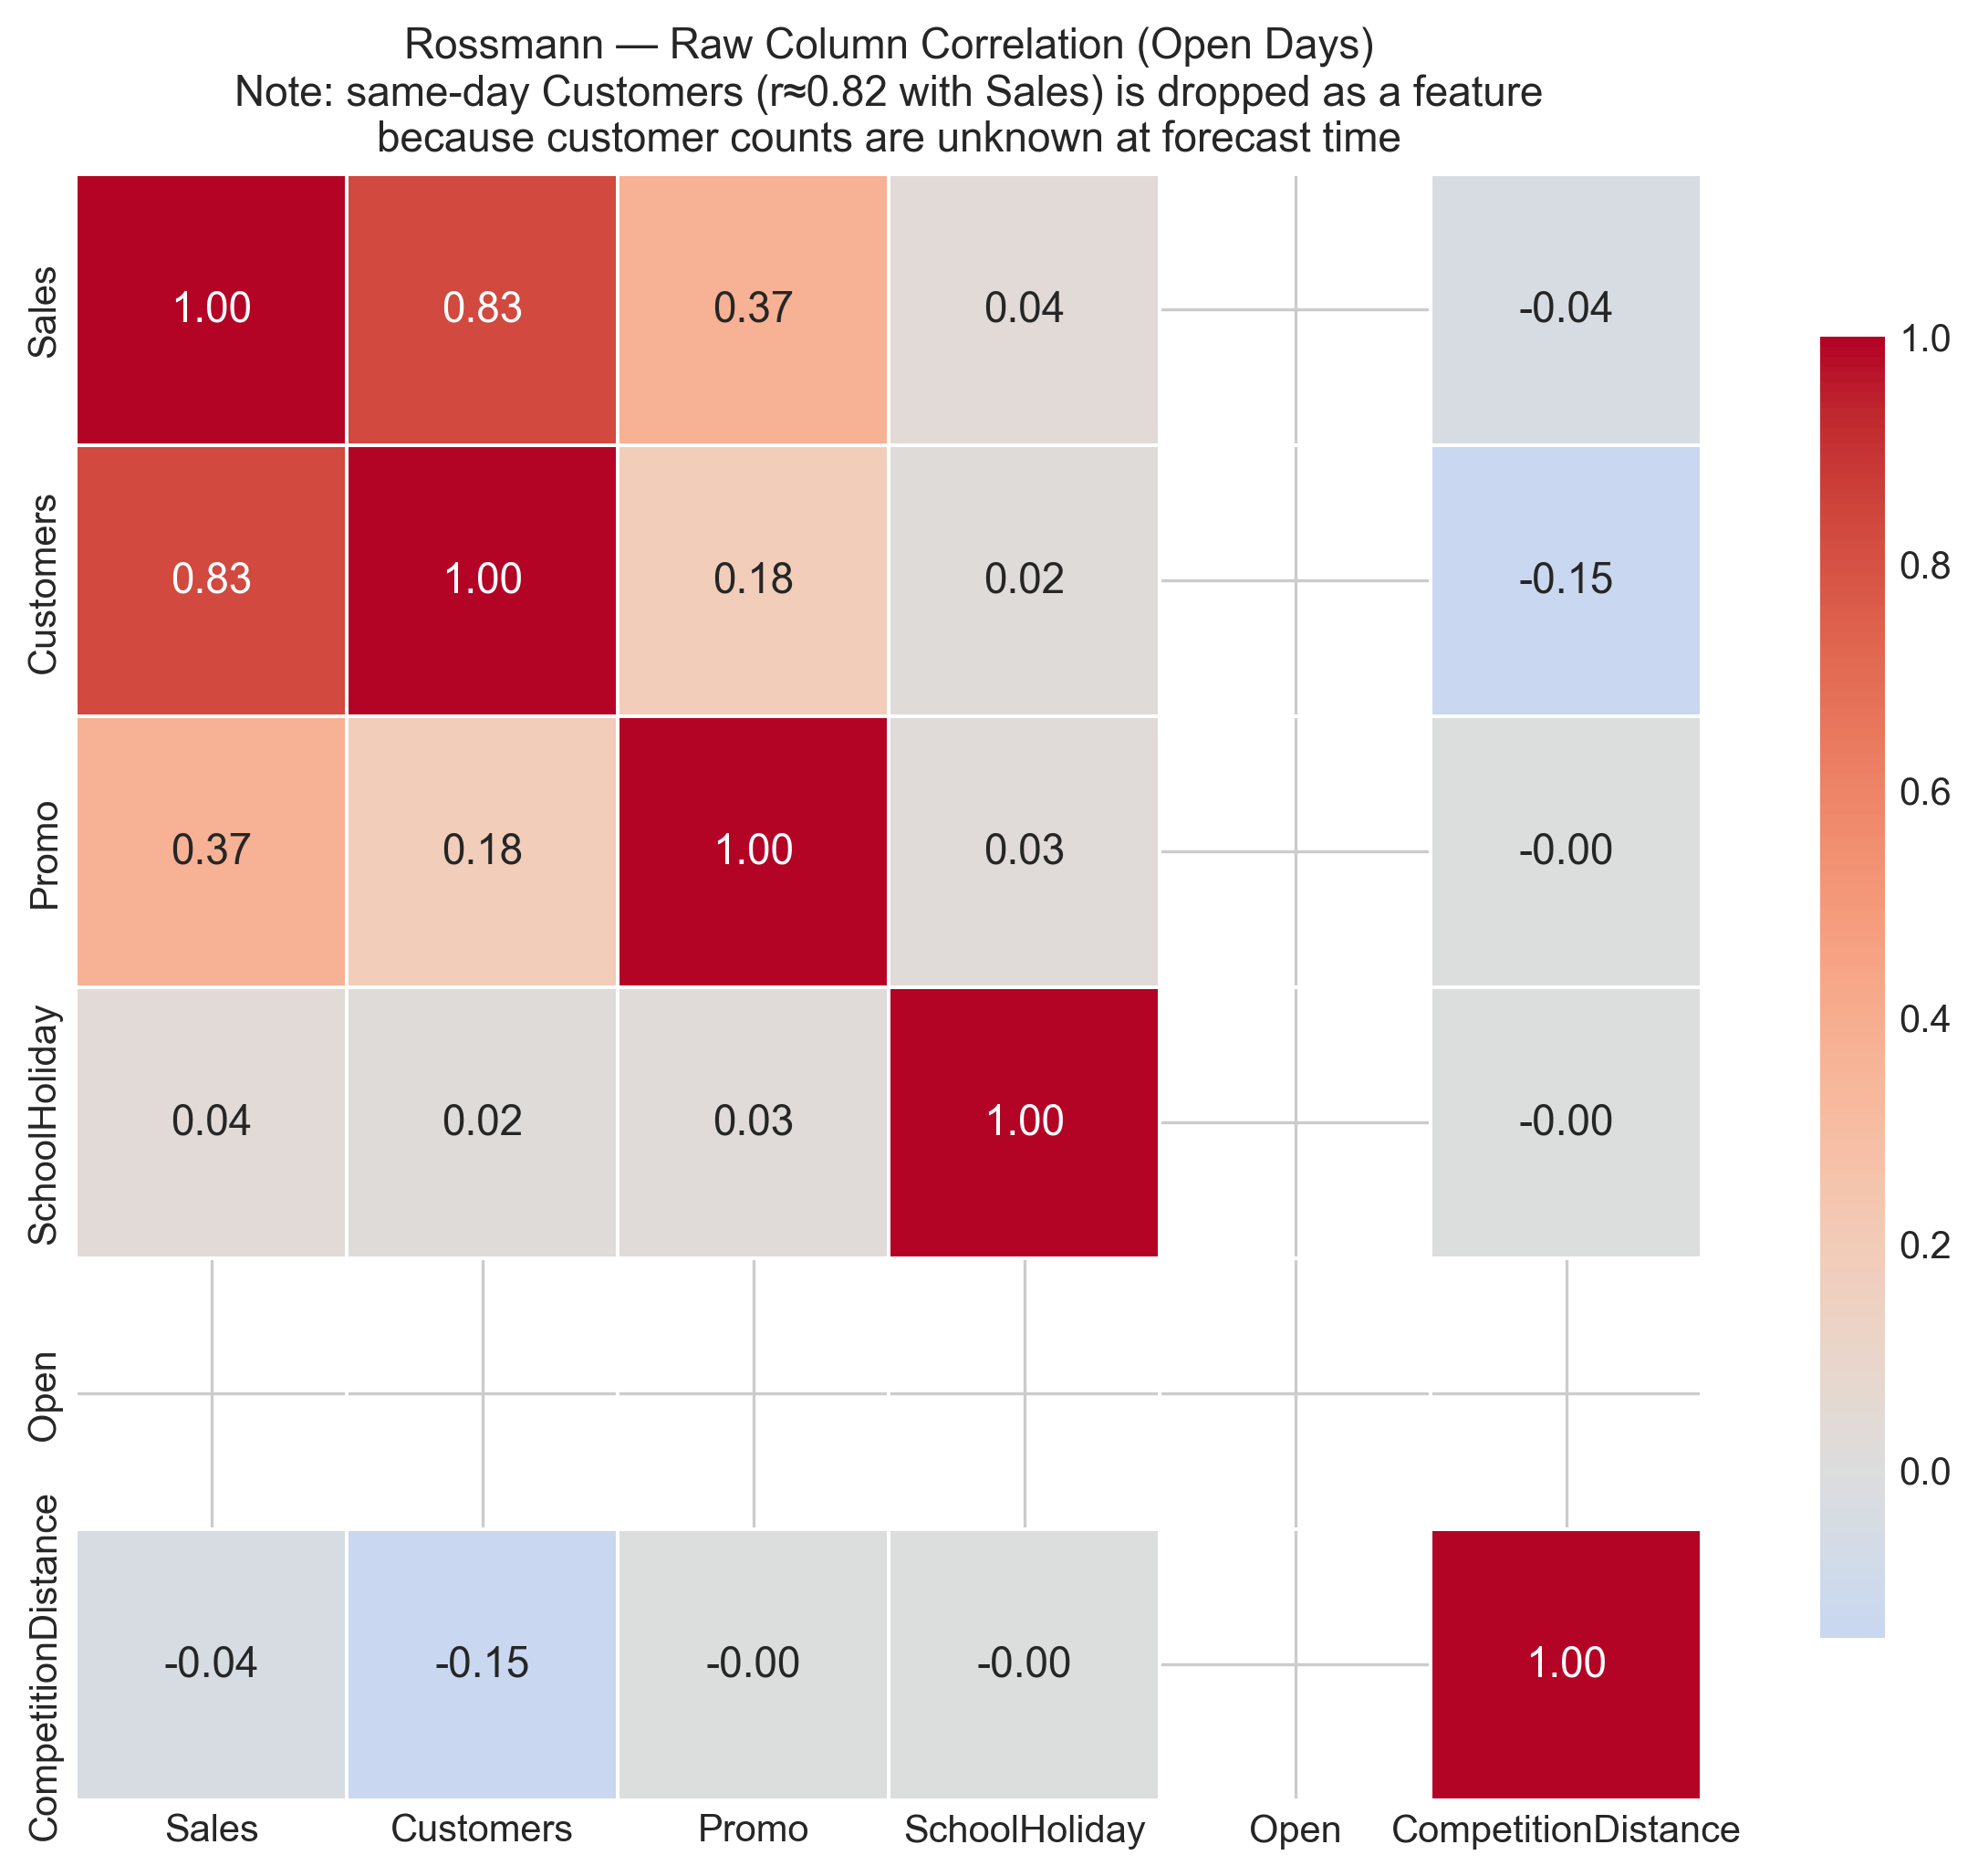
\includegraphics[width=\textwidth]{figures/rossmann_raw_correlation.png}
        \caption{Raw features correlation heatmap}
        \label{fig:rossmann_raw_corr}
    \end{subfigure}
    \hfill
    \begin{subfigure}[b]{0.48\textwidth}
        \centering
        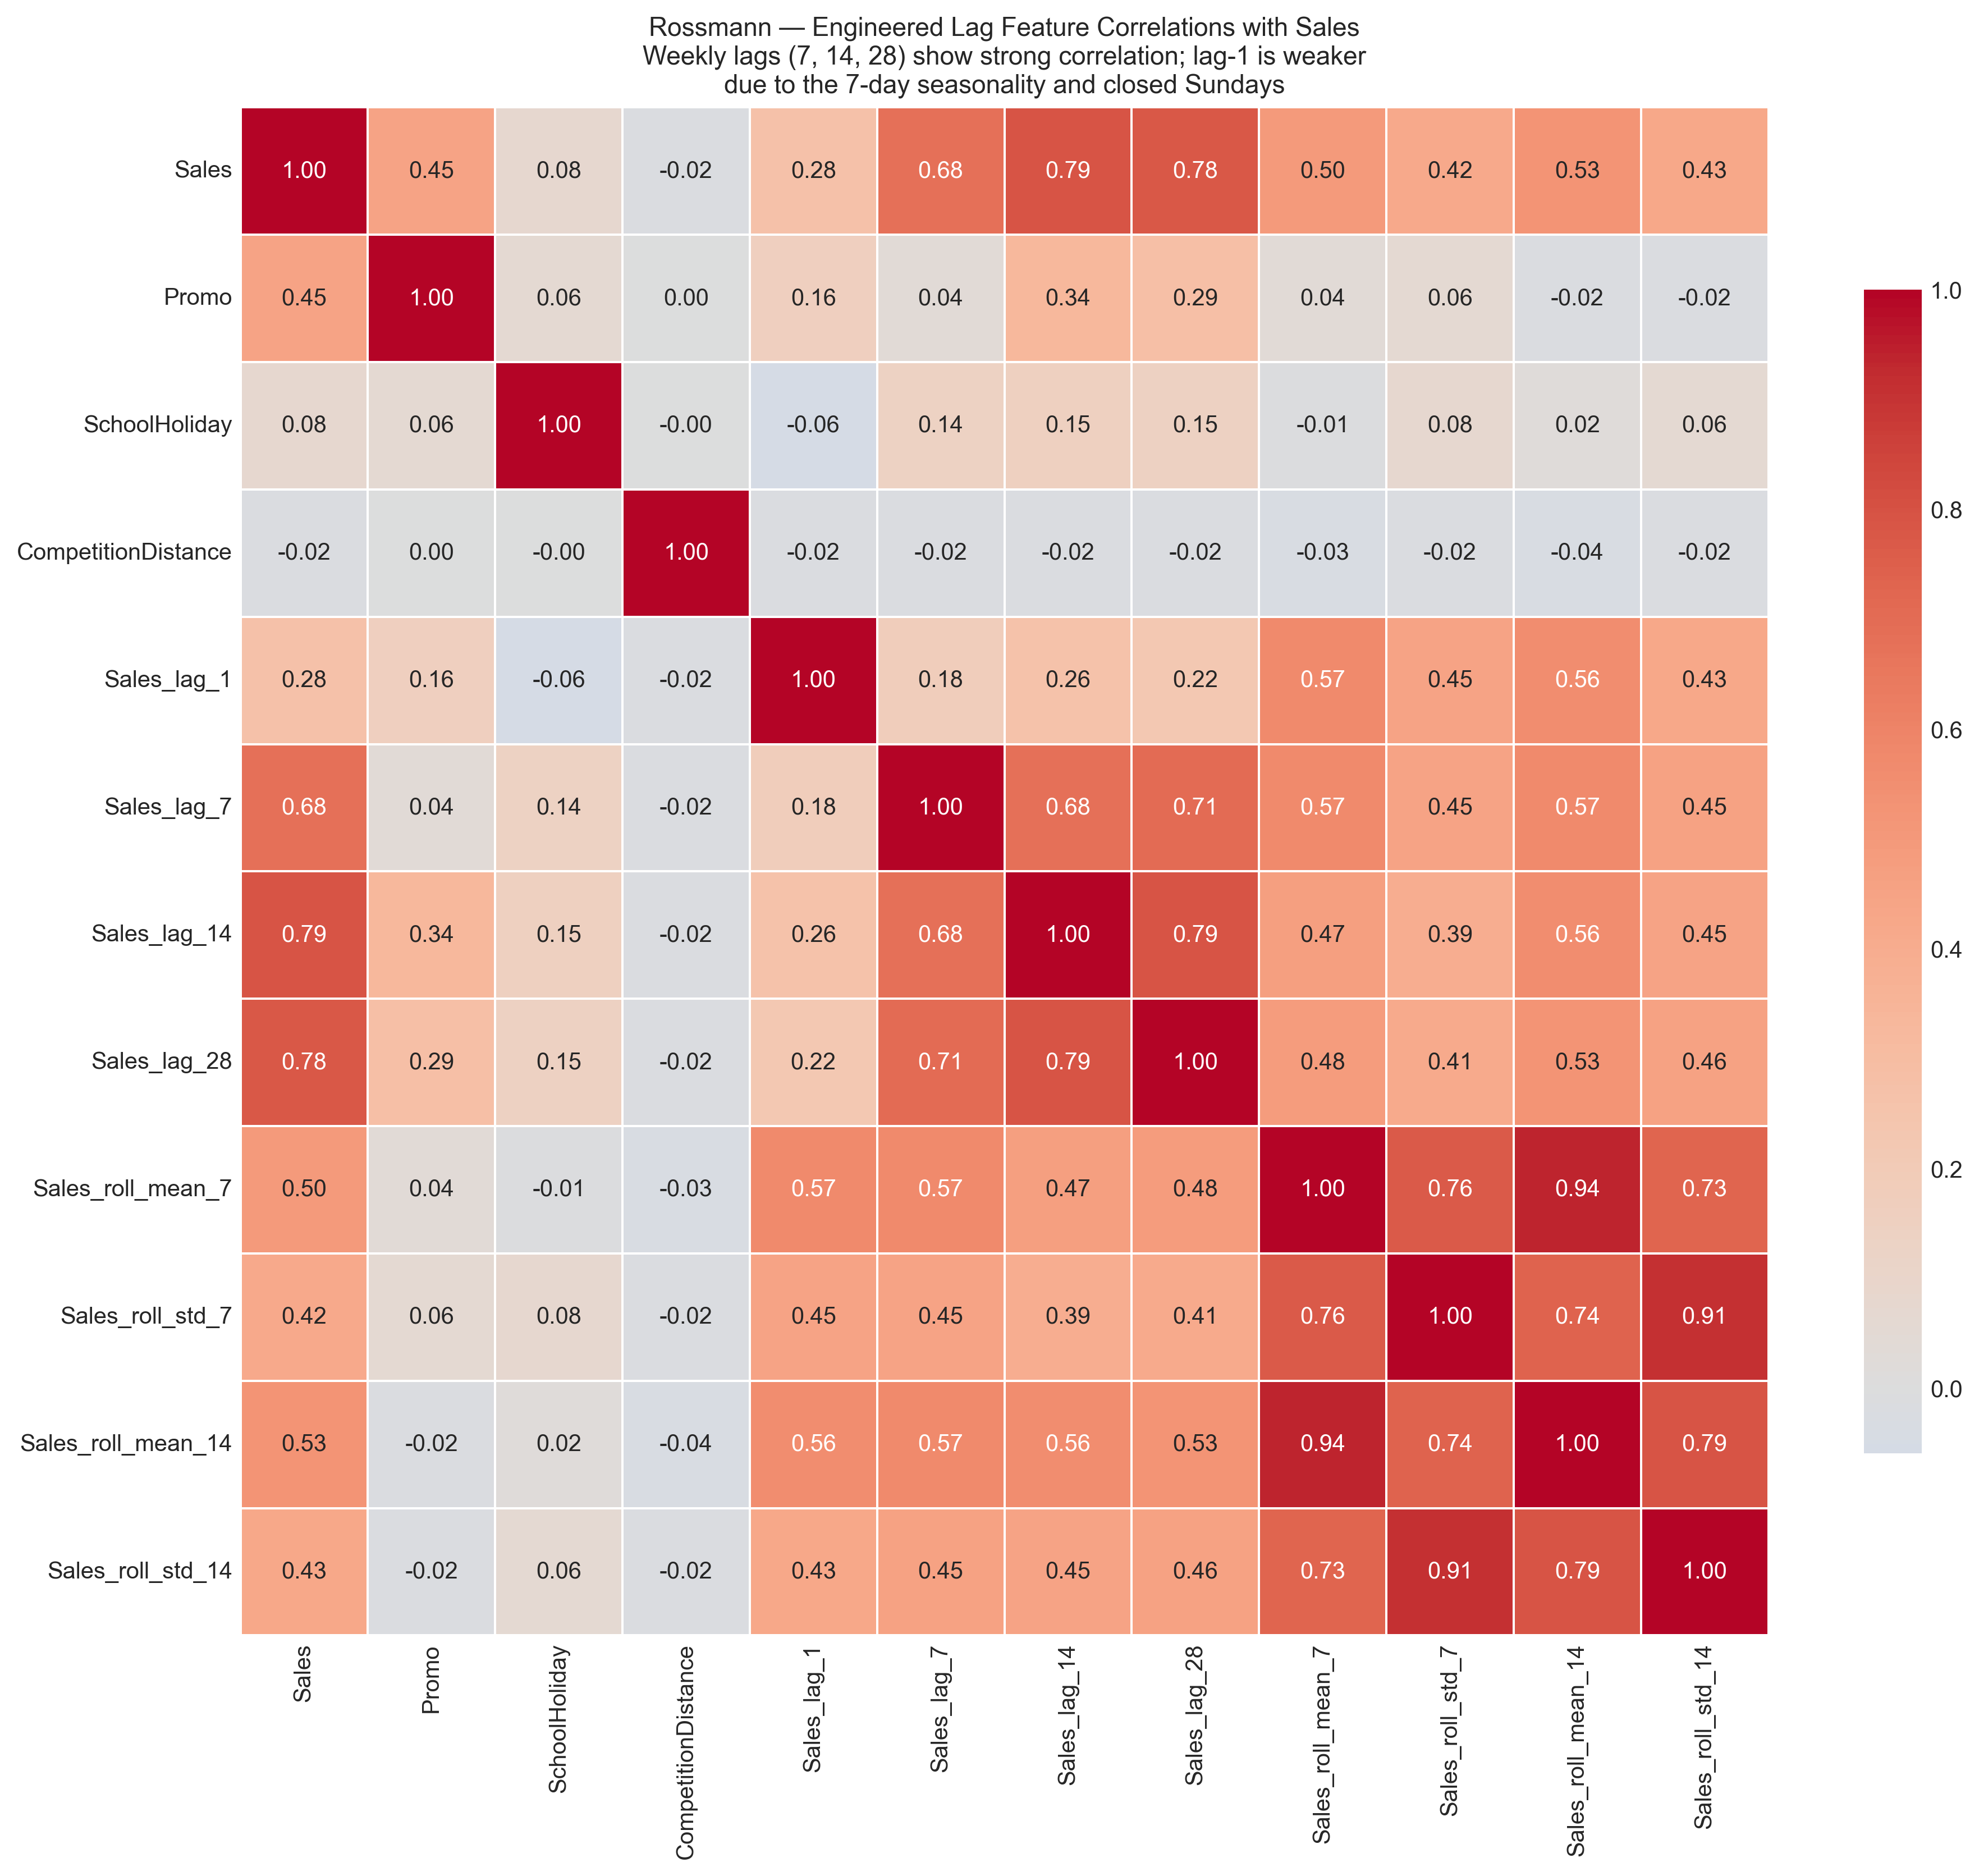
\includegraphics[width=\textwidth]{figures/rossmann_correlation_heatmap.png}
        \caption{Engineered features correlation matrix}
        \label{fig:rossmann_corr}
    \end{subfigure}
    \caption{Correlation structures for Pipeline A (Rossmann). Subfigure (b) demonstrates that lagged customer counts ($r = 0.6805$) serve as a strong predictive proxy while preserving strict forecasting validity.}
\end{figure}

\subsubsection{Autoregressive Lag Structure}
Figure \ref{fig:rossmann_lag_corr} provides an autocorrelation profile for Rossmann store sales across lags 1 through 28. The heatmap reveals recurring correlation peaks precisely at 7-day intervals (lags 7, 14, 21, and 28), confirming strong weekly periodicity and justifying our selected lag architecture.

\begin{figure}[H]
    \centering
    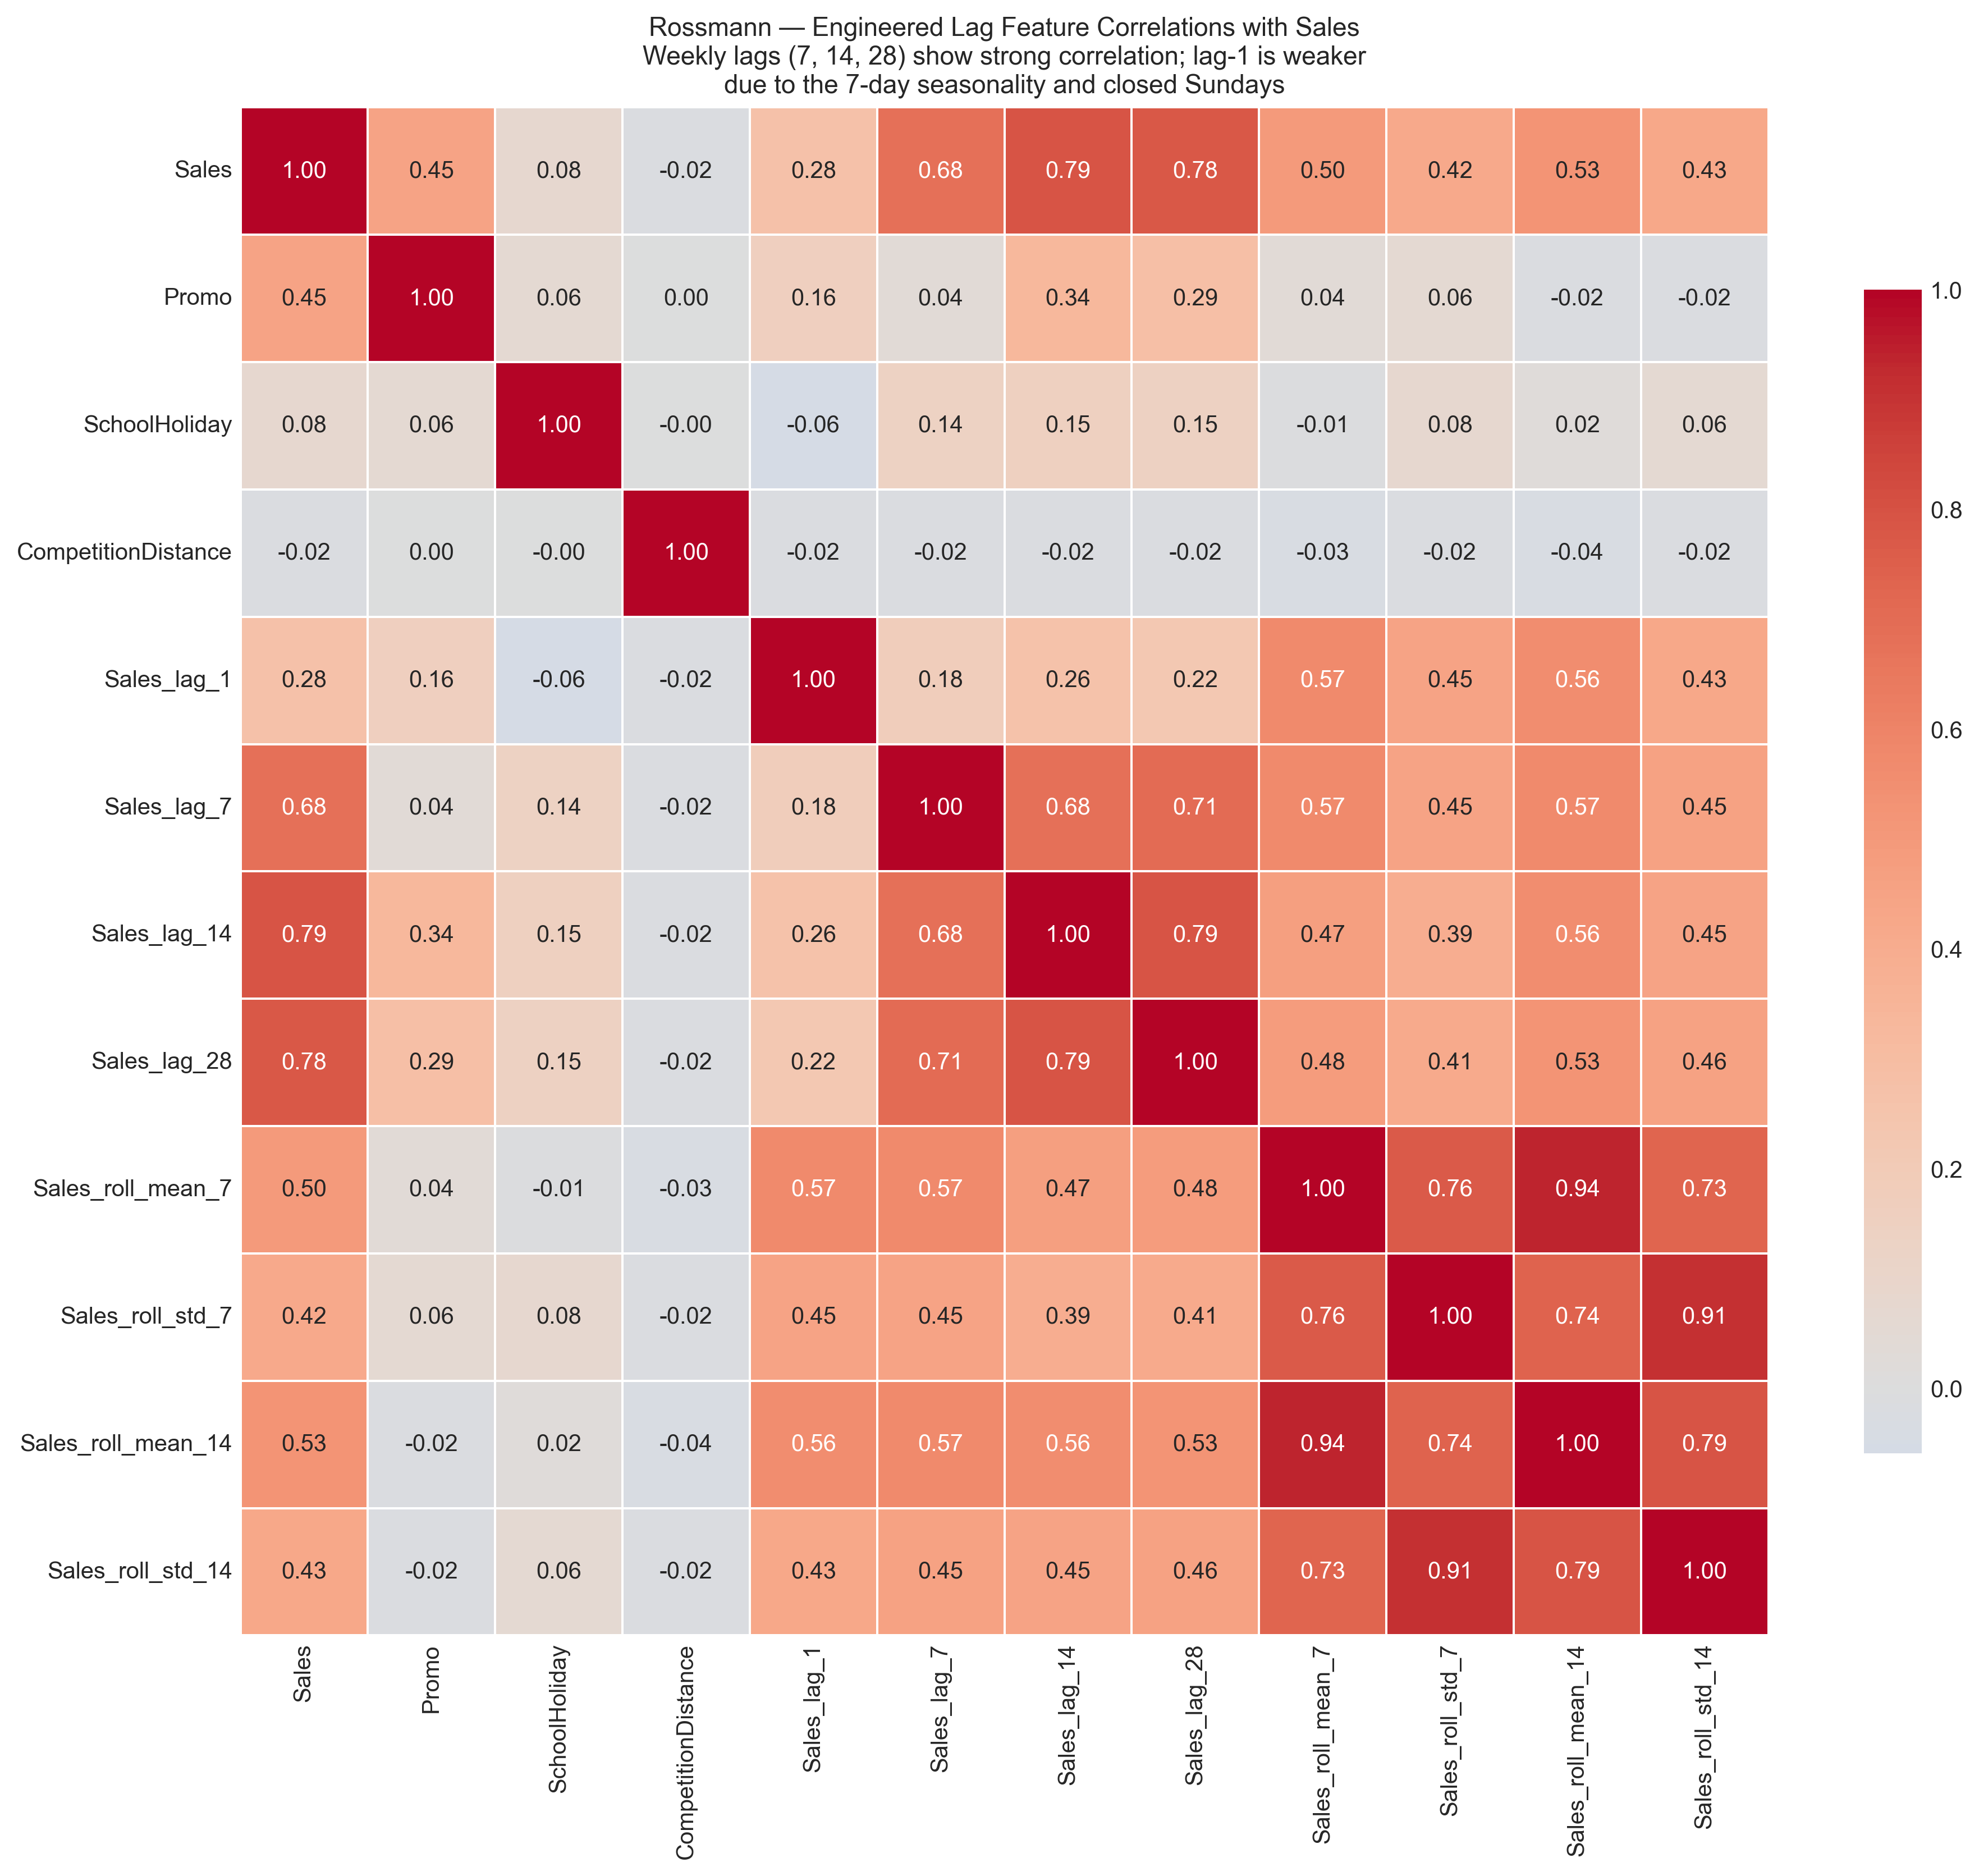
\includegraphics[width=0.75\textwidth]{figures/rossmann_lag_correlation.png}
    \caption{Autoregressive correlation profile of Rossmann sales across lags 1 to 28, illustrating pronounced resonance at multi-week intervals ($7, 14, 21, 28$).}
    \label{fig:rossmann_lag_corr}
\end{figure}

\FloatBarrier
\newpage

\subsection{Store Item Demand Dynamics}

\subsubsection{Demand Distribution and Profile}
Pipeline B contains daily unit sales across 500 individual series. Across all 913,000 records, unit sales average \textbf{52.23 units} ($\sigma = 28.77$, median = 47.0, range = 0 to 200). Figure \ref{fig:store_item_hist} illustrates the unimodal distribution of item sales, while Figure \ref{fig:store_item_zeros} confirms that zero-demand events occurred only once in five years (0.0001\%), demonstrating that every series maintains continuous non-intermittent turnover.

\begin{figure}[H]
    \centering
    \begin{subfigure}[b]{0.48\textwidth}
        \centering
        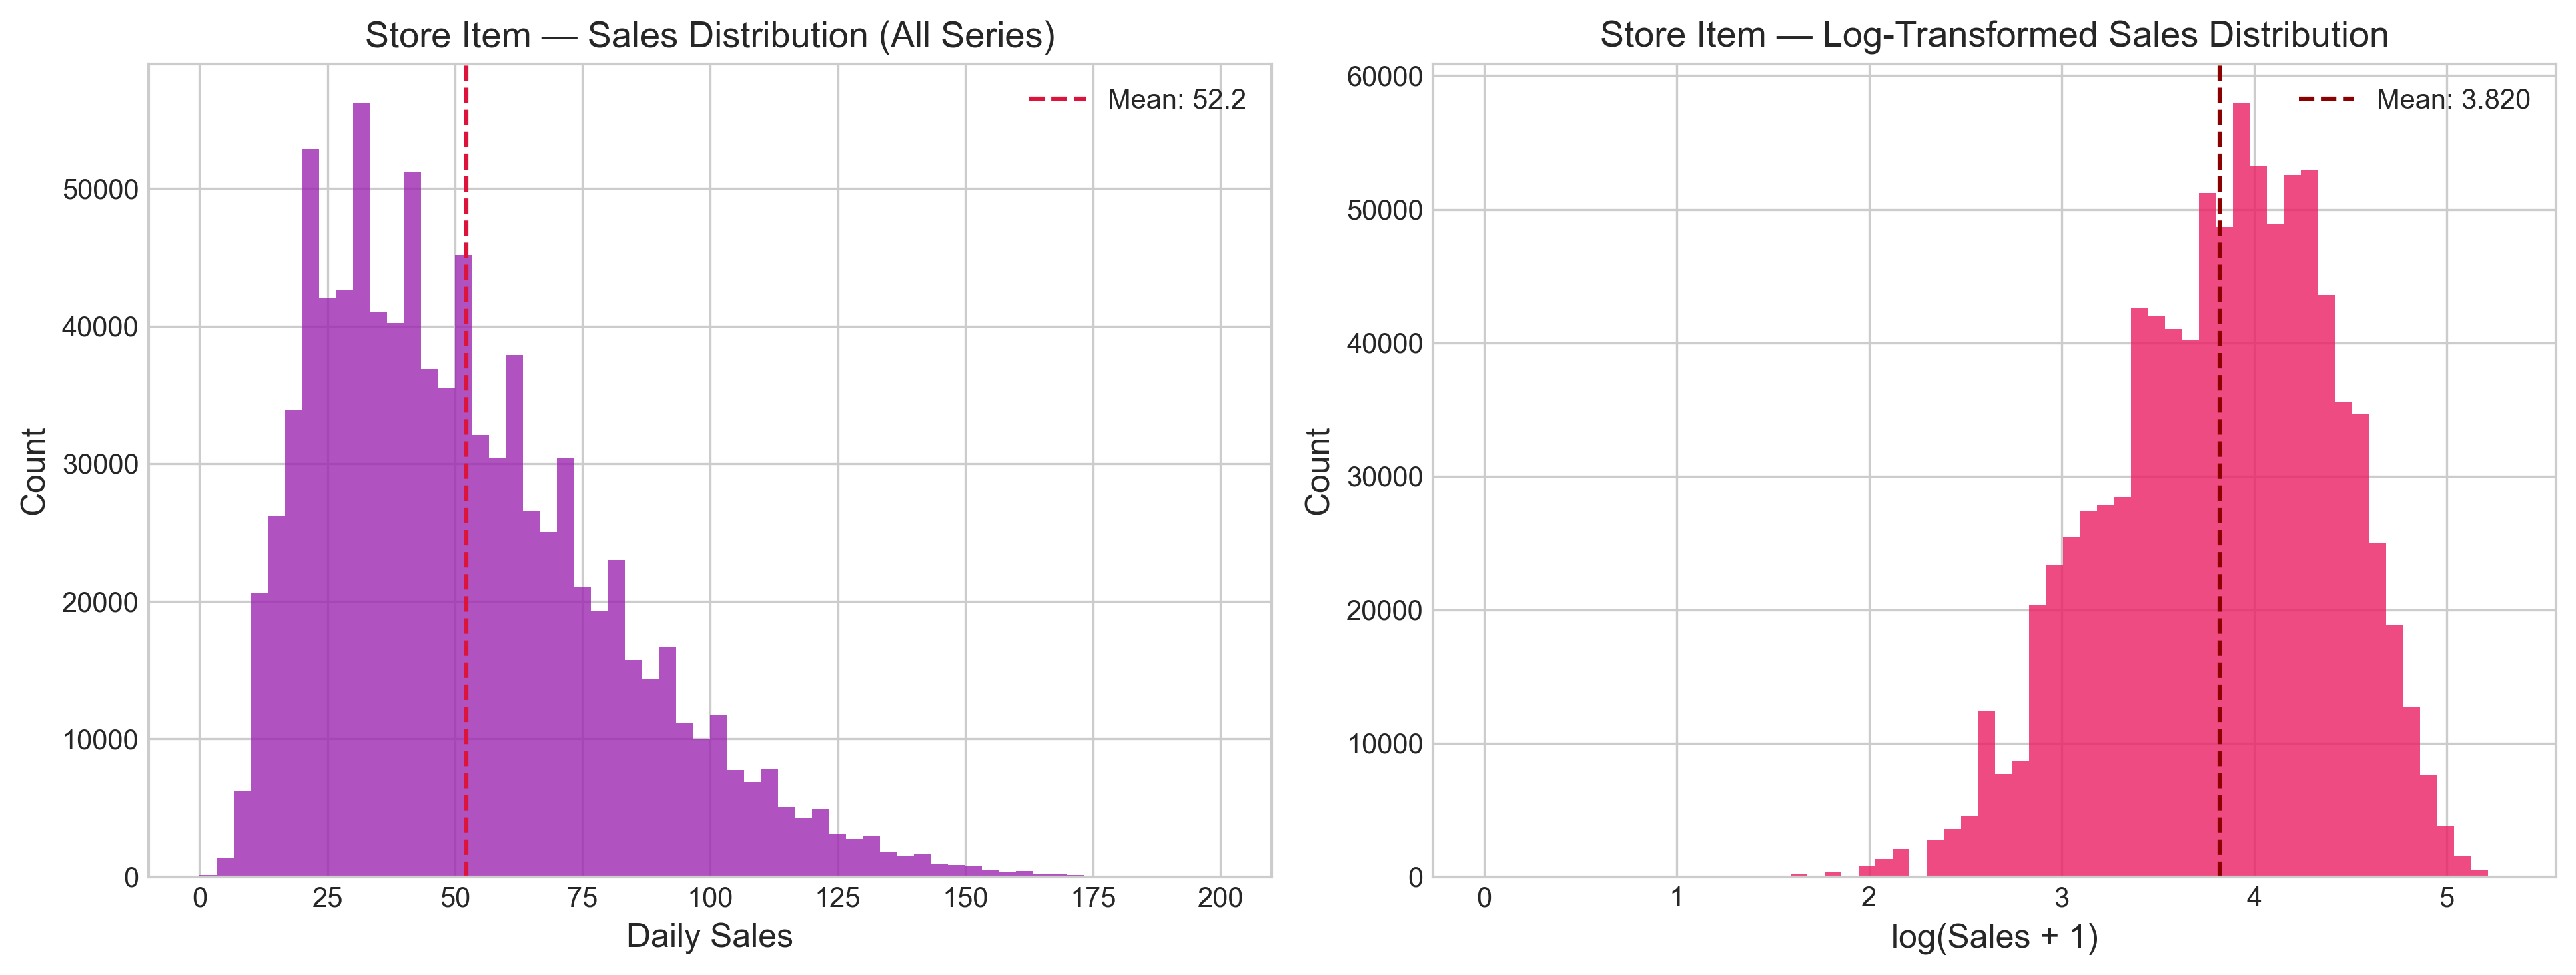
\includegraphics[width=\textwidth]{figures/store_item_sales_histogram.png}
        \caption{Daily unit demand distribution}
        \label{fig:store_item_hist}
    \end{subfigure}
    \hfill
    \begin{subfigure}[b]{0.48\textwidth}
        \centering
        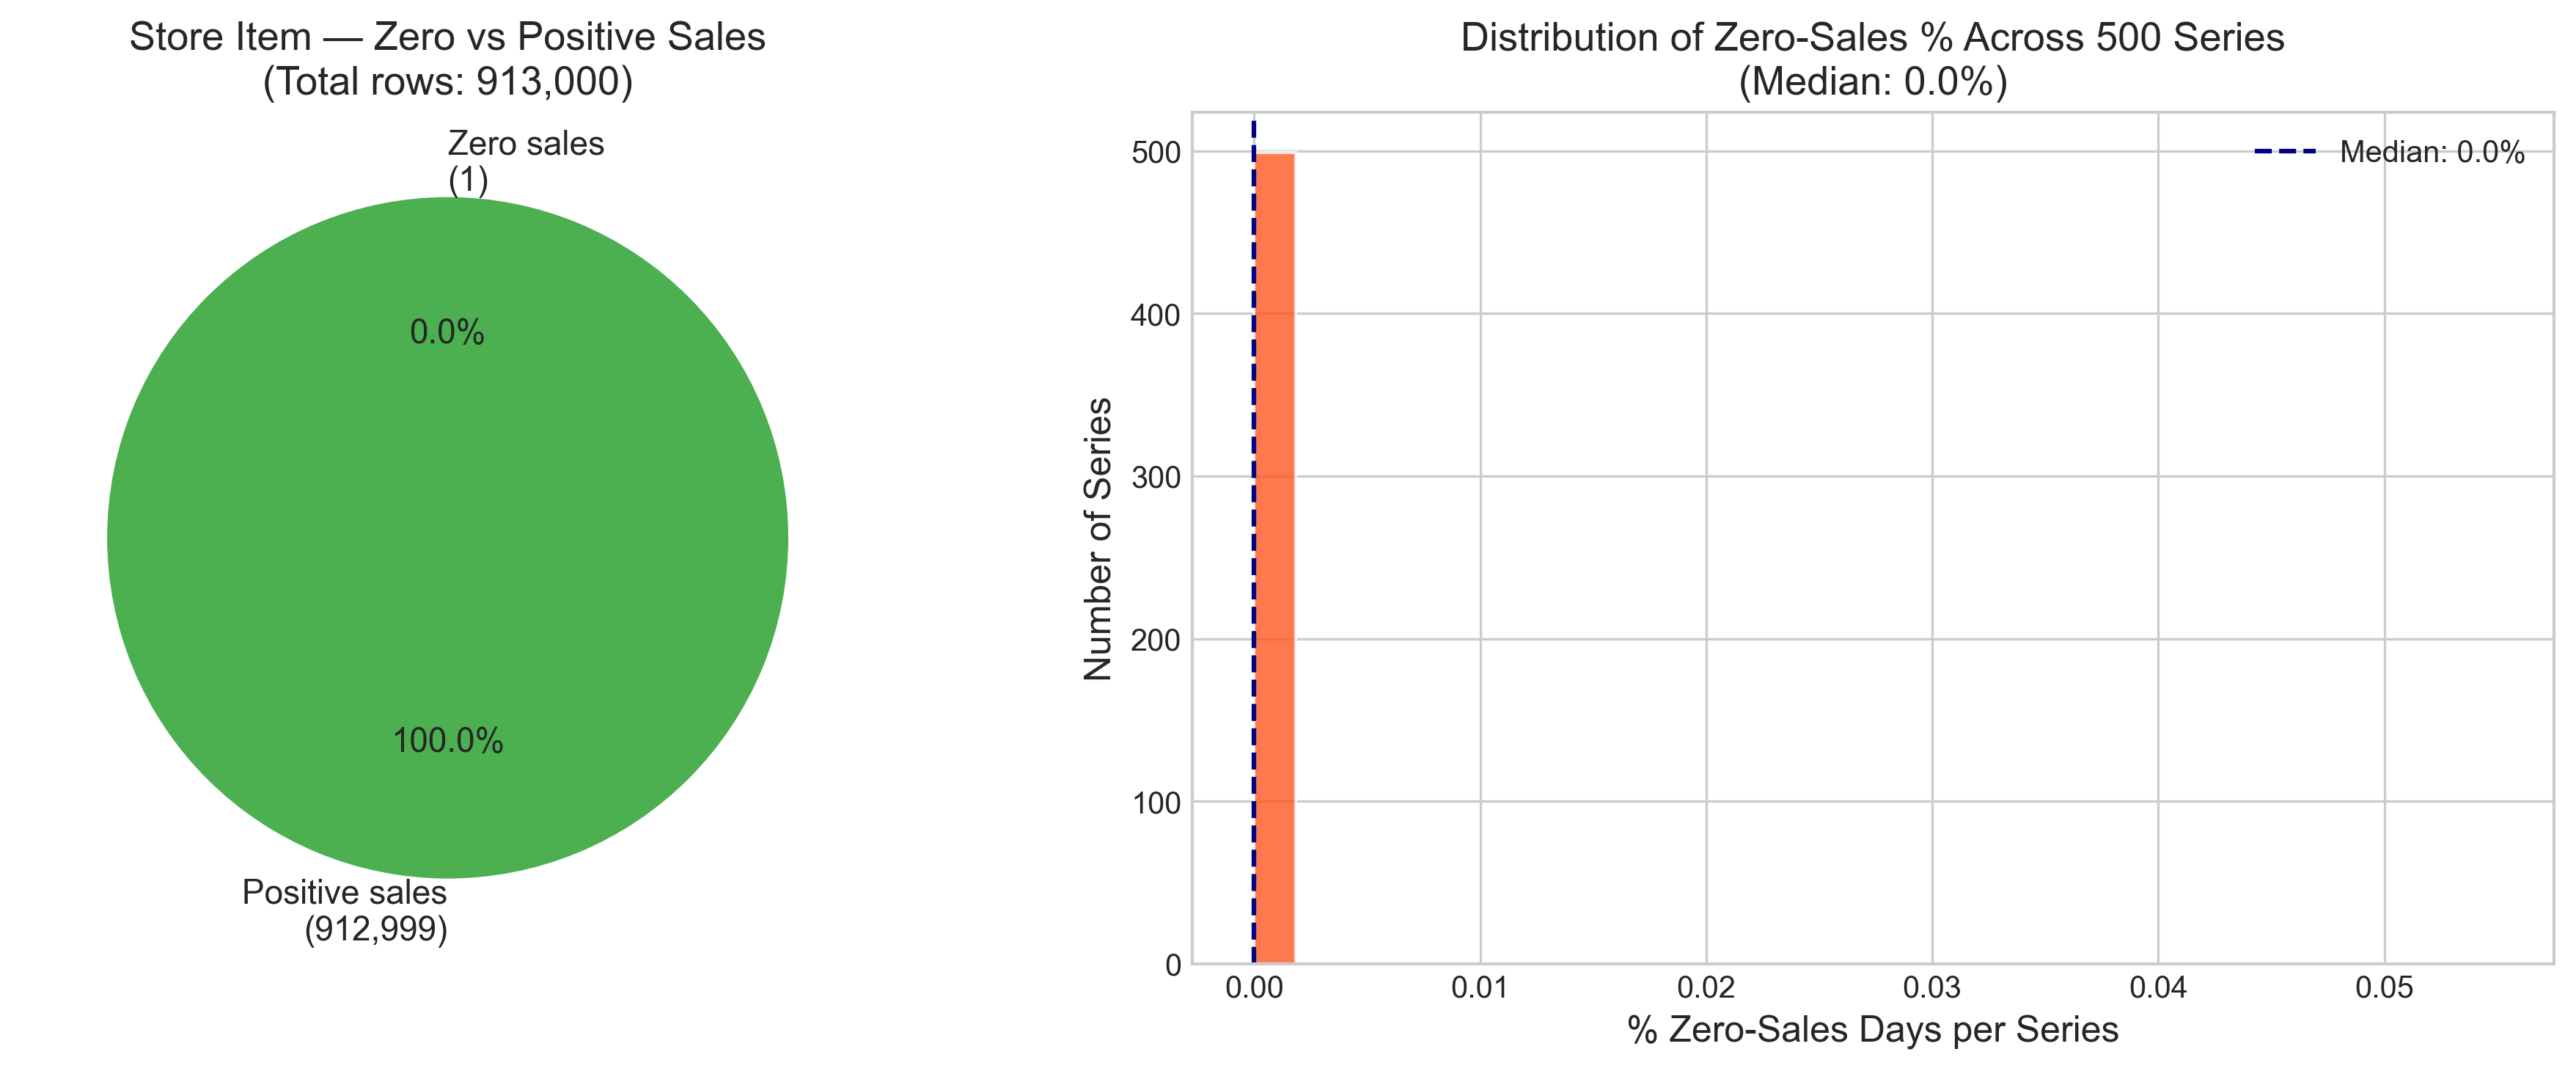
\includegraphics[width=\textwidth]{figures/store_item_zero_summary.png}
        \caption{Zero-demand incidence analysis}
        \label{fig:store_item_zeros}
    \end{subfigure}
    \caption{Distributional properties of Store Item demand (Pipeline B).}
\end{figure}

\subsubsection{Weekly and Annual Seasonality Profiles}
Figure \ref{fig:store_item_dow} depicts the day-of-week demand profile across all 10 stores. Demand follows a consistent weekly rhythm across all stores, climbing steadily from Monday (lowest demand, $\approx 38$ units) to a peak on Sunday ($\approx 68$ units).

Figure \ref{fig:store_item_month} depicts the monthly seasonality profile, revealing a smooth annual sinusoidal progression that peaks during the summer months (July mean $\approx 64$ units) and troughs in winter (January mean $\approx 37$ units). Figure \ref{fig:store_item_season} displays five-year longitudinal trajectories for representative series, showing steady annual growth combined with recurring seasonal waves.

\begin{figure}[H]
    \centering
    \begin{subfigure}[b]{0.48\textwidth}
        \centering
        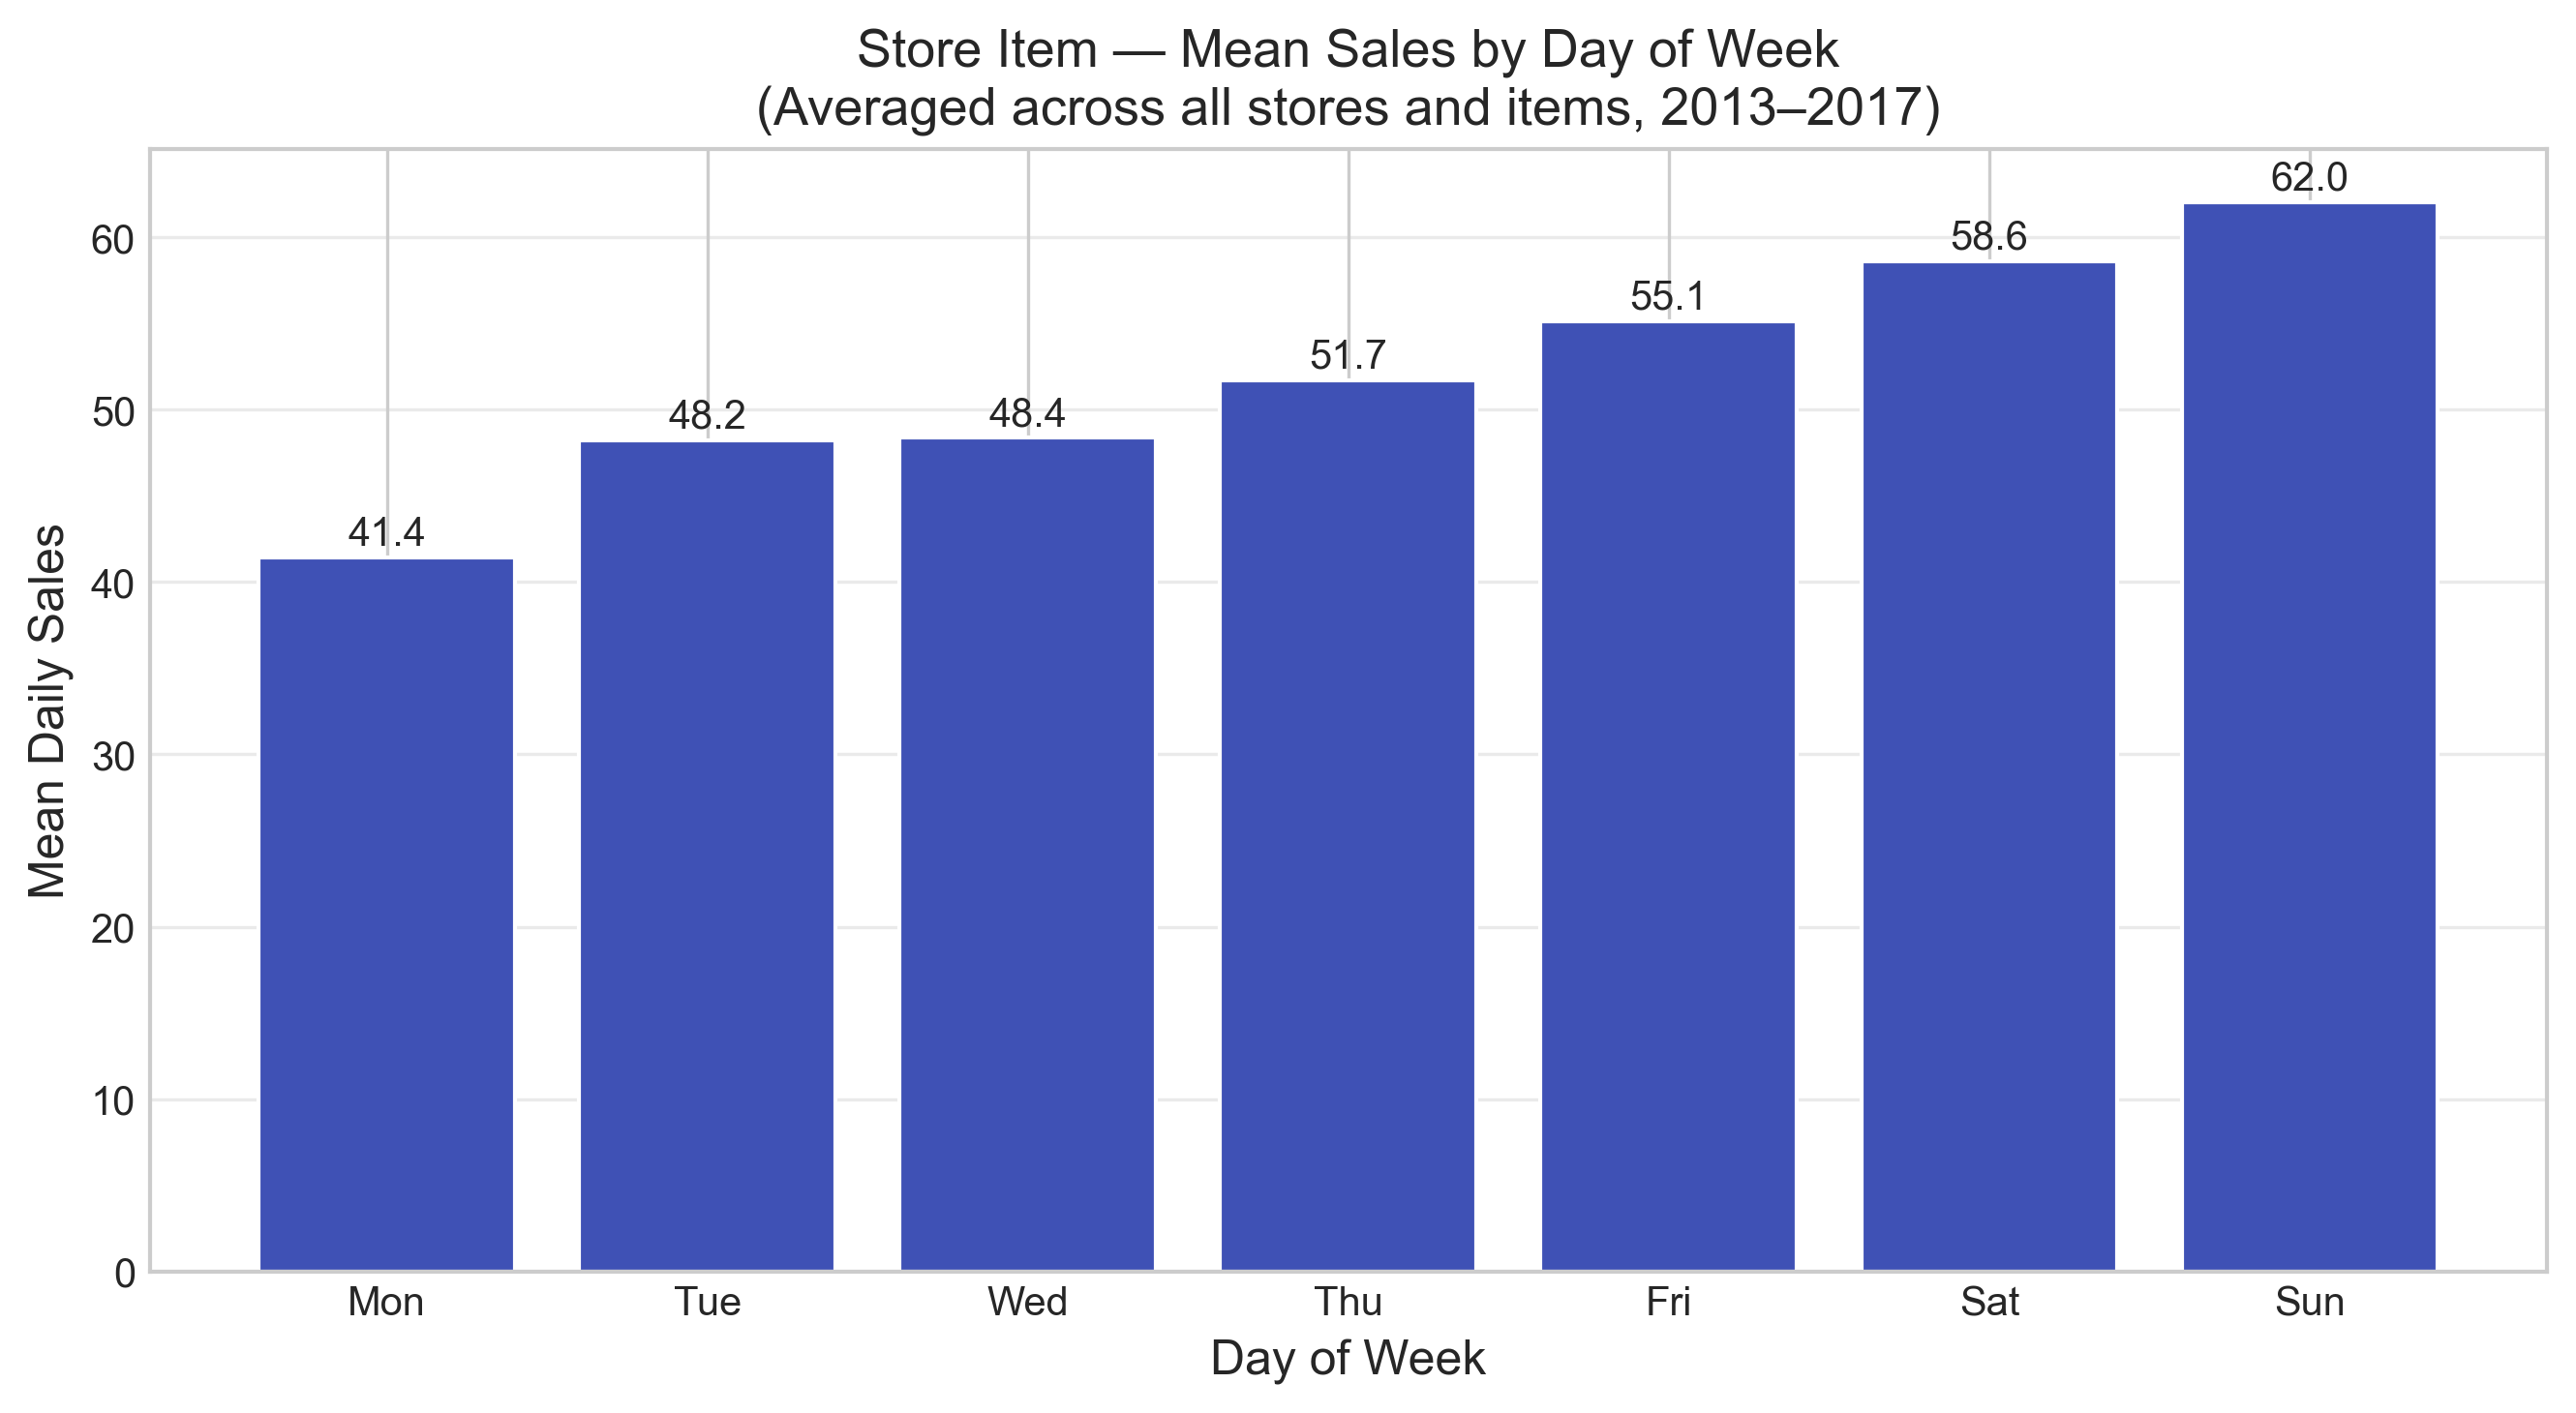
\includegraphics[width=\textwidth]{figures/store_item_dow_profile.png}
        \caption{Day-of-week sales profile by store}
        \label{fig:store_item_dow}
    \end{subfigure}
    \hfill
    \begin{subfigure}[b]{0.48\textwidth}
        \centering
        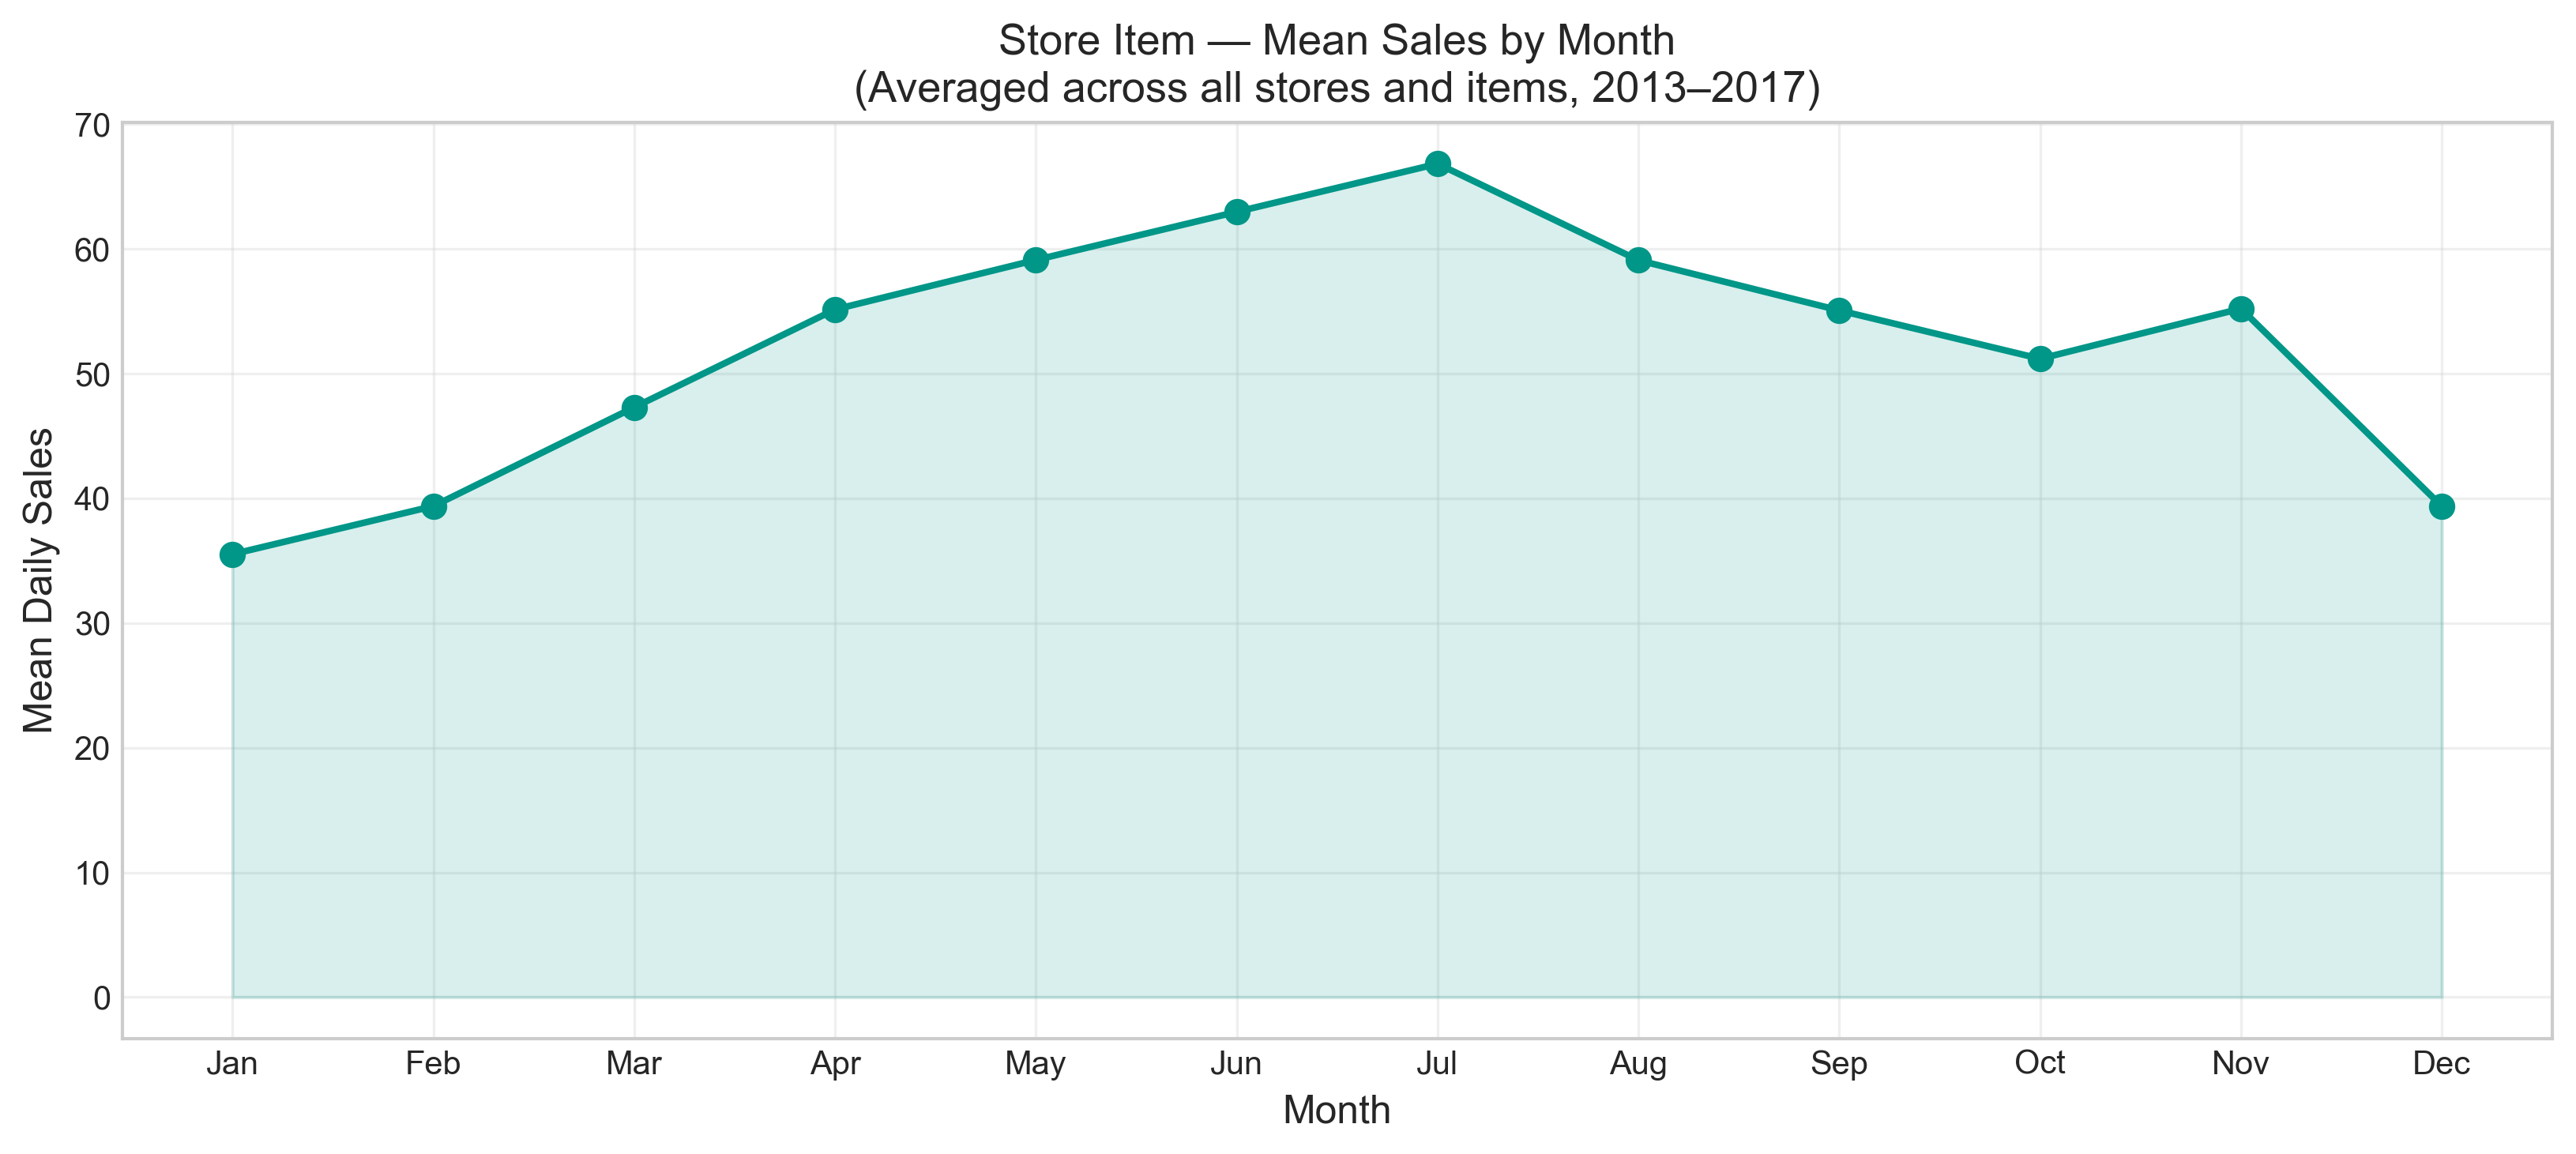
\includegraphics[width=\textwidth]{figures/store_item_monthly_profile.png}
        \caption{Monthly seasonality progression}
        \label{fig:store_item_month}
    \end{subfigure}
    \caption{Temporal seasonality profiles for Pipeline B across all 10 stores.}
\end{figure}

\begin{figure}[H]
    \centering
    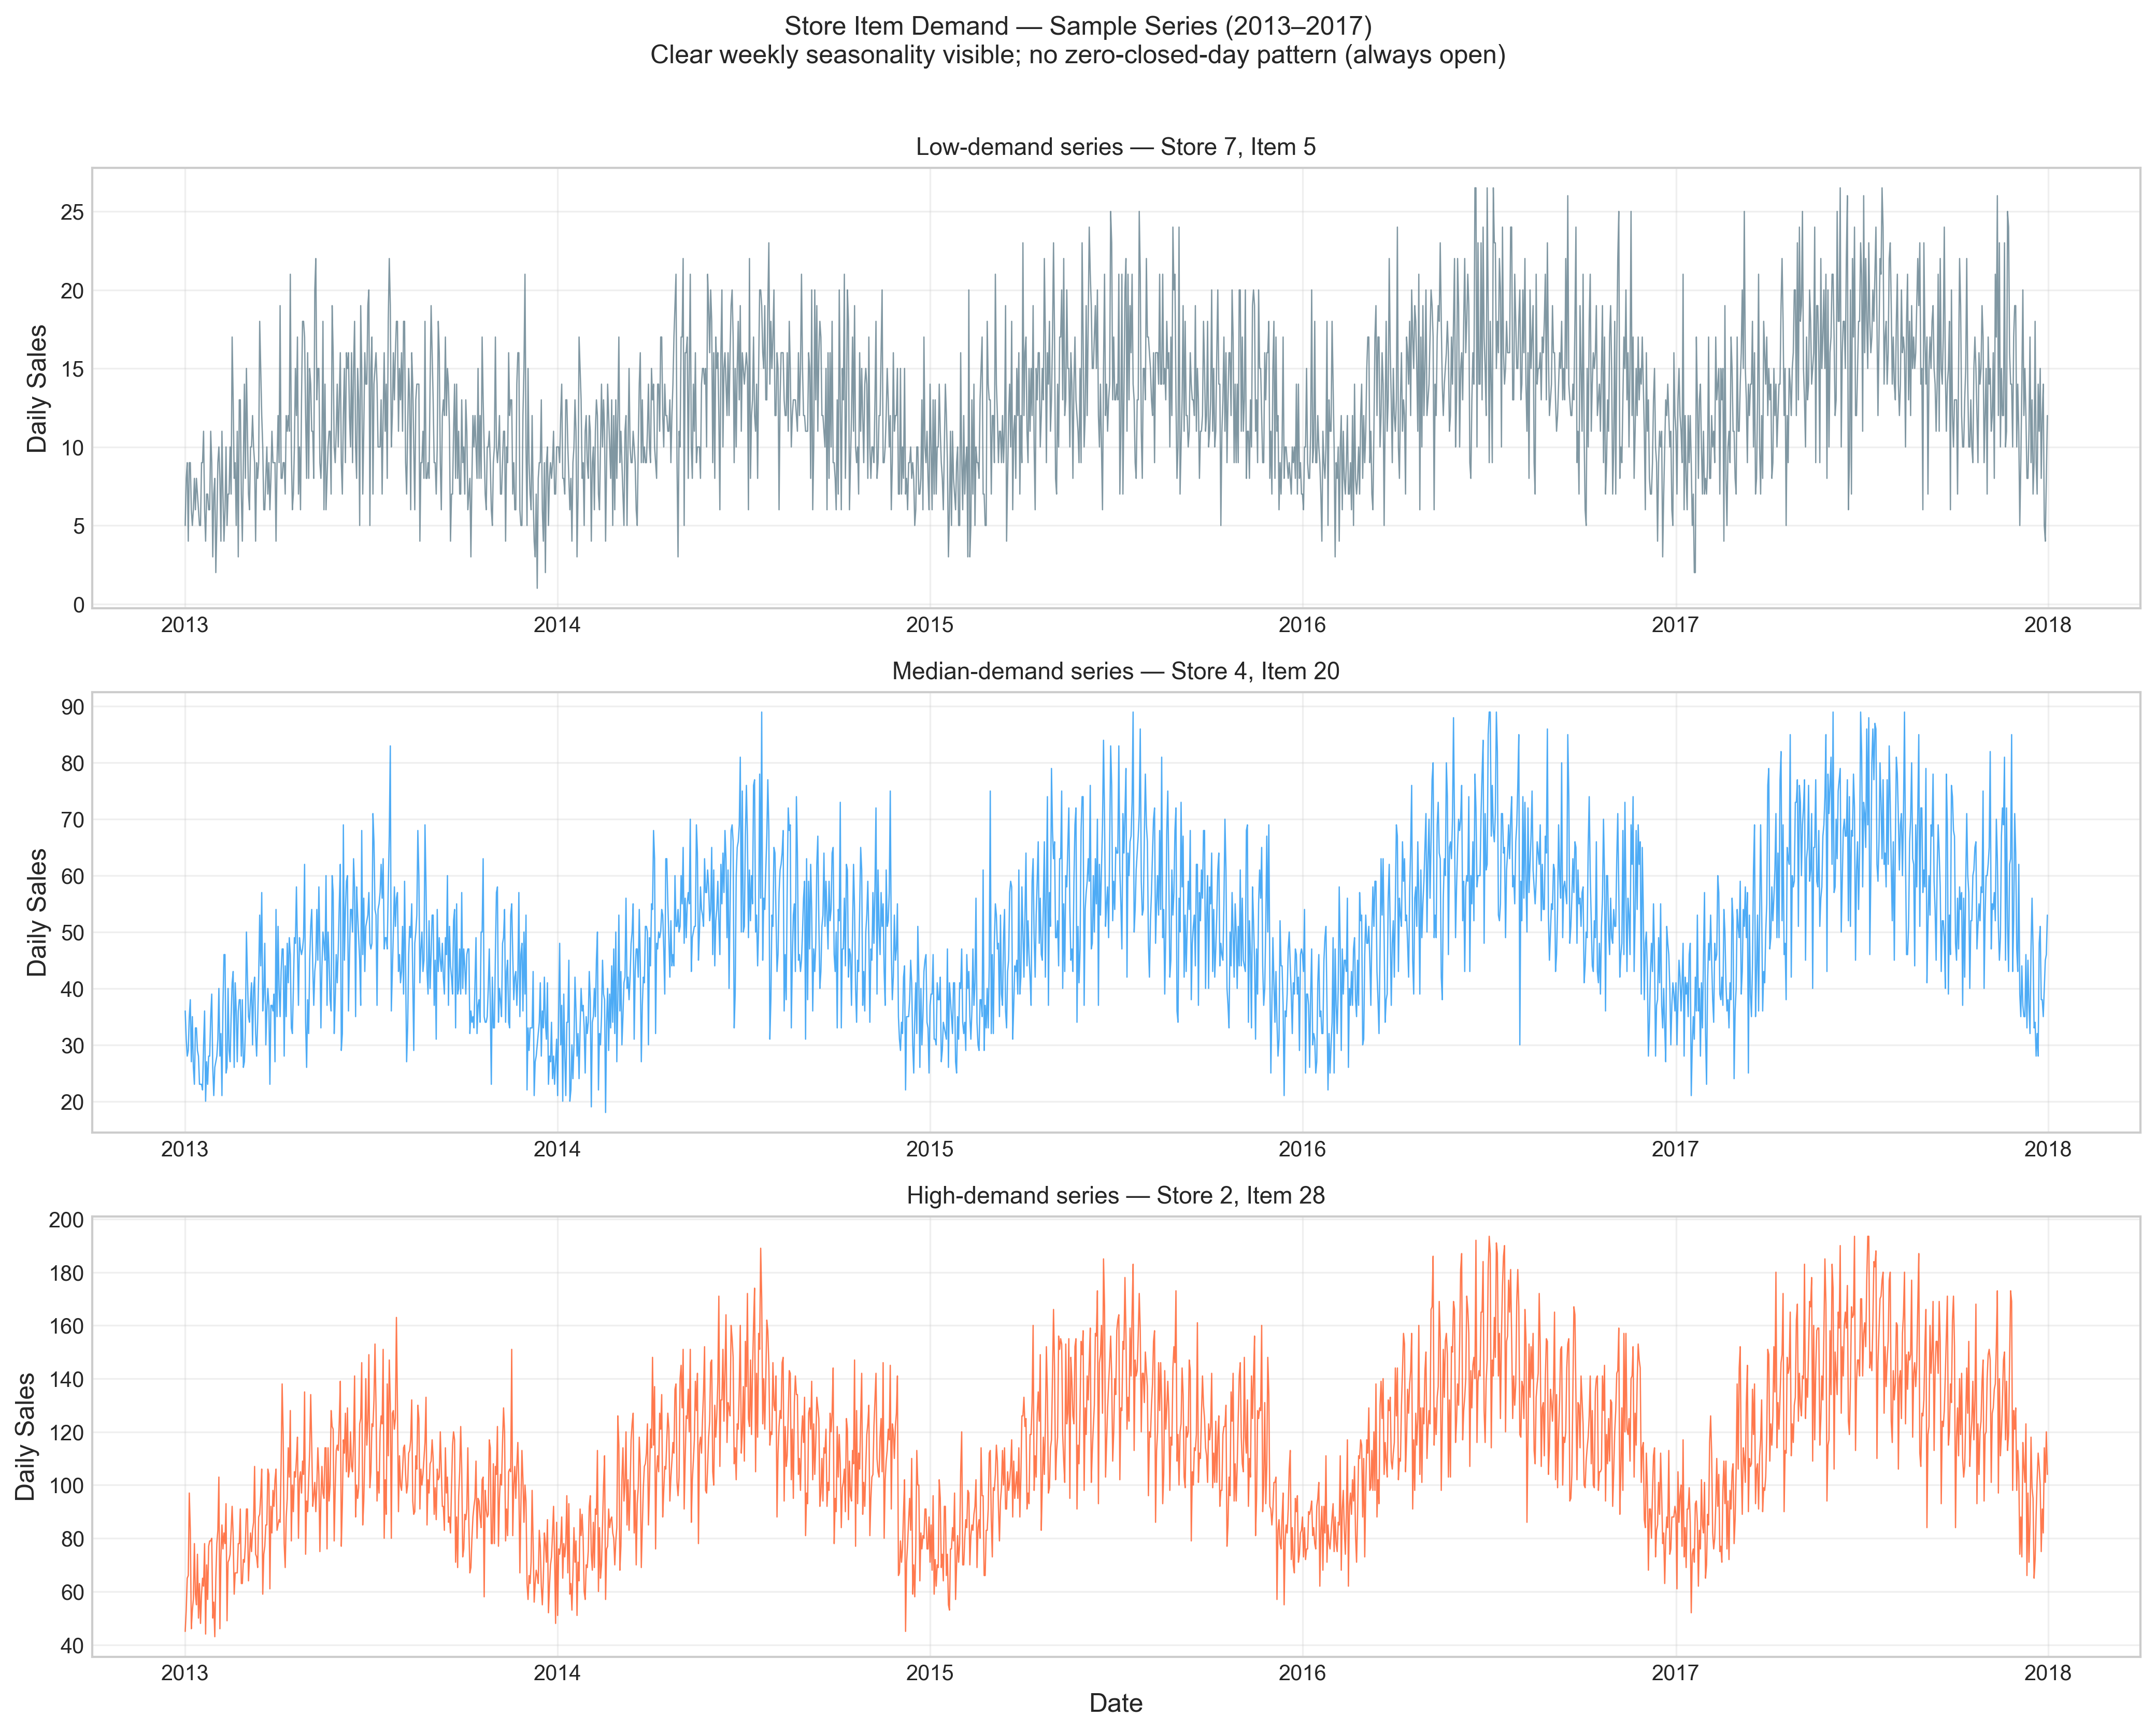
\includegraphics[width=0.9\textwidth]{figures/store_item_seasonality.png}
    \caption{Five-year historical sales trajectories for sample store--item series, highlighting robust multi-year annual seasonality and volume differences.}
    \label{fig:store_item_season}
\end{figure}

\FloatBarrier
\newpage

\subsection{Time-Based Split Validation Schema}
Figure \ref{fig:time_split} illustrates the time-based holdout validation design implemented across both pipelines. In contrast to random cross-validation, which introduces temporal lookahead leakage, the time-based holdout strictly partitions the chronological axis: the model trains on historical data and is tested against an unseen contiguous future horizon (42 days for Rossmann, 90 days for Store Item).

\begin{figure}[H]
    \centering
    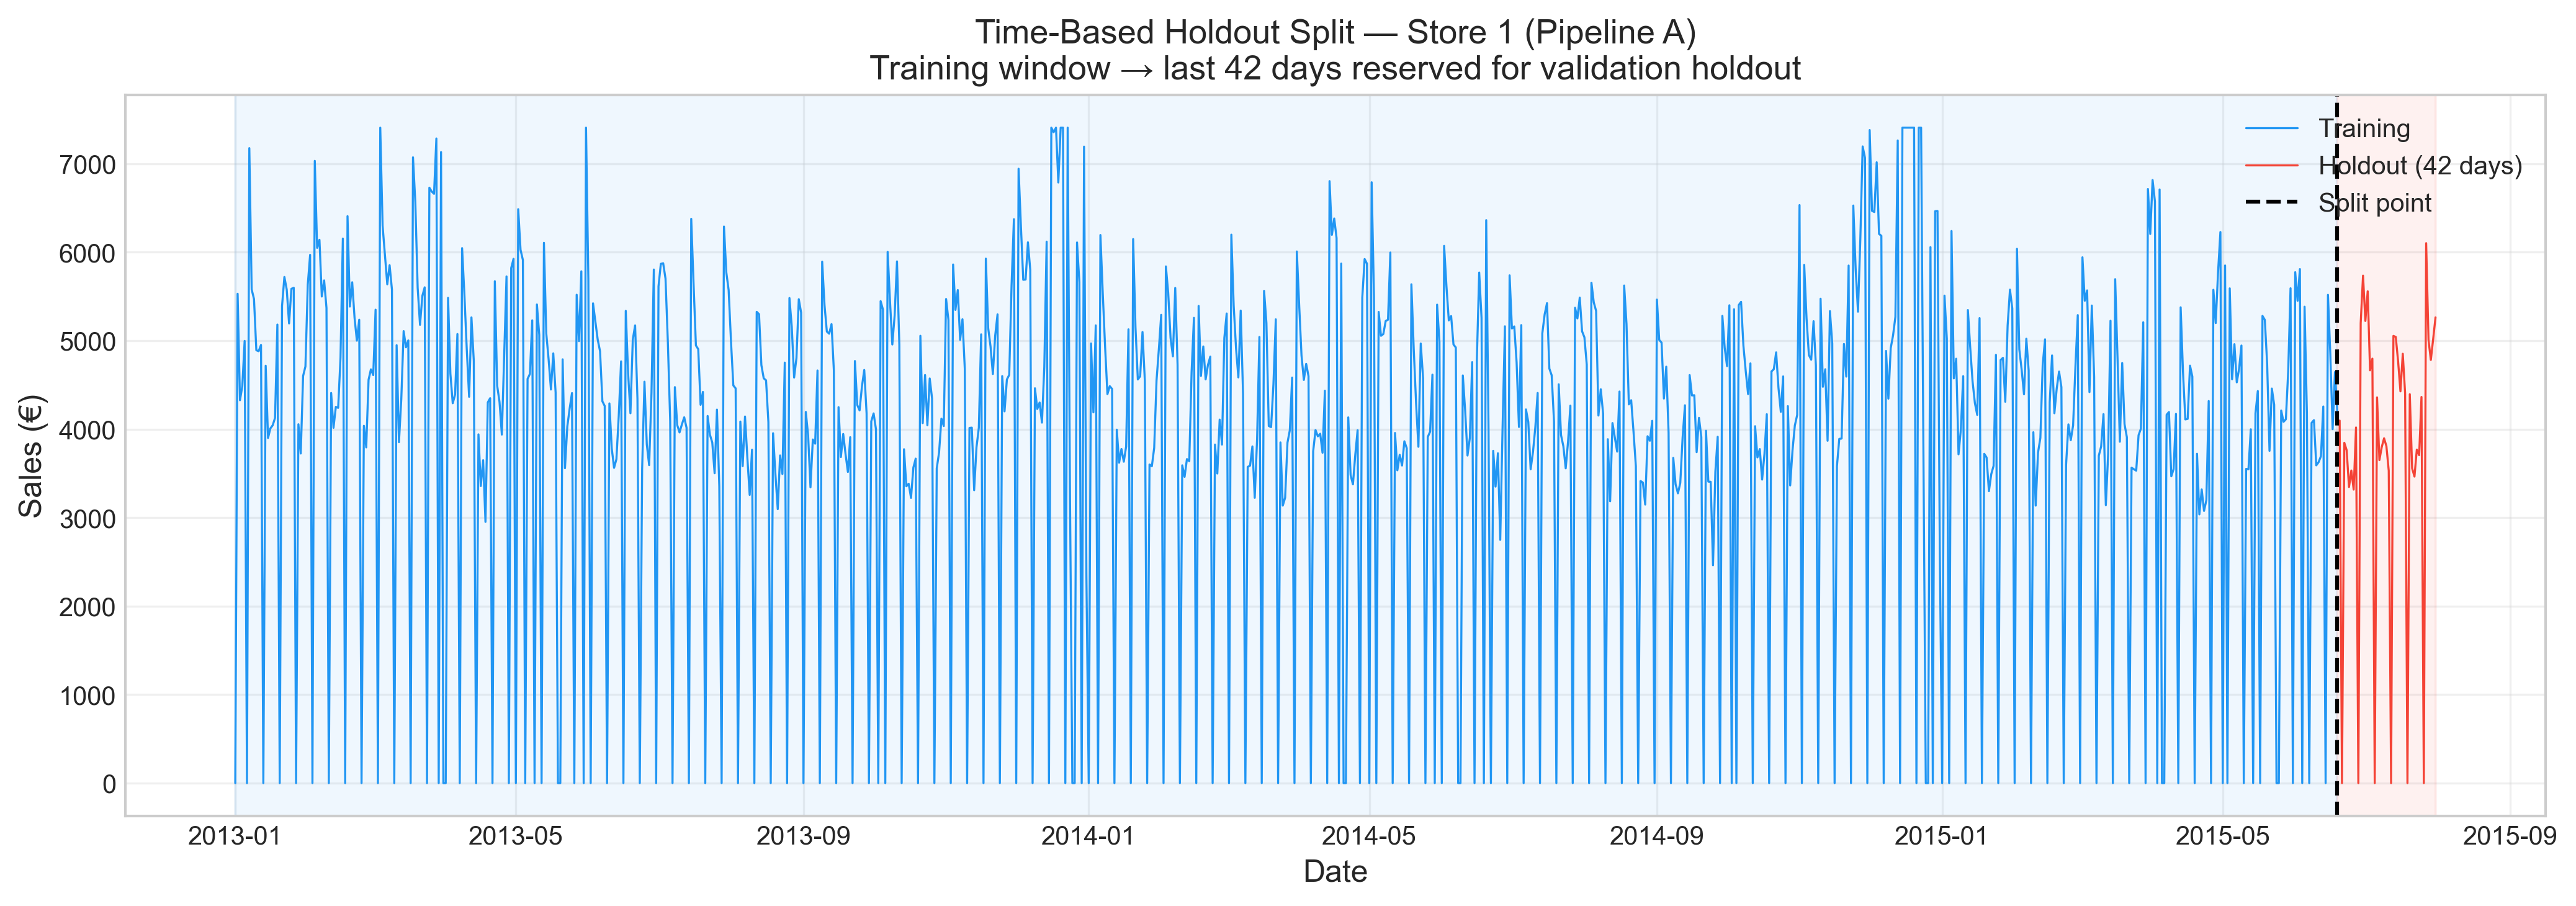
\includegraphics[width=0.88\textwidth]{figures/time_based_split_diagram.png}
    \caption{Time-based holdout split strategy: training window with 28-day lag warm-up buffer followed by a contiguous future validation holdout, ensuring zero leakage.}
    \label{fig:time_split}
\end{figure}

\FloatBarrier

\section{Summary of Deliverable 1 Contributions}

Deliverable 1 establishes the problem formulation and data foundations for the project:
\begin{enumerate}
    \item \textbf{Concrete Problem Definition:} Formulated the business trade-off between stockouts and inventory holding costs, defined target users, and provided technical justifications for machine-learning-driven uncertainty estimation over static heuristic rules.
    \item \textbf{Dual Pipeline Separation:} Implemented two parallel, unmerged data pipelines representing store-level multivariate demand (Rossmann) and multi-item SKU demand (Store Item).
    \item \textbf{Reproducible Data Pipeline:} Built an automated execution sequence (\texttt{run\_all.py}) covering programmatic acquisition, schema validation, domain rule enforcement, leakage-safe outlier treatment, and feature generation.
    \item \textbf{Leakage Prevention:} Enforced strict chronological splitting (42-day Rossmann holdout, 90-day Store Item holdout), withheld contemporaneous customer volume, and computed all normalization parameters solely on training partitions.
    \item \textbf{Visual EDA:} Generated and analyzed 10 high-resolution visualizations characterizing promotional lift (+38.4\%), weekly and annual periodicity, and autoregressive lag correlations.
\end{enumerate}

\FloatBarrier
\newpage

\begin{thebibliography}{9}

\bibitem{rossmann_kaggle}
Rossmann, \emph{Rossmann Store Sales: Forecast sales using store, promotion, and competitor data}, Kaggle Competition, 2015. \url{https://www.kaggle.com/c/rossmann-store-sales}

\bibitem{store_item_kaggle}
Kaggle, \emph{Store Item Demand Forecasting Challenge: Predict 3 months of demand for 50 different items at 10 different stores}, Kaggle Competition, 2018. \url{https://www.kaggle.com/c/demand-forecasting-kernels-only}

\bibitem{ke2017lightgbm}
G.~Ke, Q.~Meng, T.~Finley, T.~Wang, W.~Chen, W.~Ma, Q.~Ye, and T.-Y.~Liu, ``LightGBM: A highly efficient gradient boosting decision tree,'' in \emph{Advances in Neural Information Processing Systems (NeurIPS 2017)}, vol.~30, pp.~3146--3154, 2017.

\end{thebibliography}

\FloatBarrier
\newpage

\appendix

\section{Empirical Data Summaries}

\subsection{Data Cleaning and Preprocessing Summary}
Table \ref{tab:cleaning_summary} provides the exact data counts from \texttt{data/processed/cleaning\_report.json} obtained by executing \texttt{02\_clean\_and\_validate.py}.

\begin{table}[H]
    \centering
    \small
    \begin{tabular}{lrr}
        \toprule
        \textbf{Pipeline Quality Metric} & \textbf{Pipeline A: Rossmann} & \textbf{Pipeline B: Store Item} \\
        \midrule
        Raw Acquired Rows & 1,017,209 & 913,000 \\
        Rows After Metadata Merge & 1,017,209 & --- \\
        Failed Date Parses & 0 & 0 \\
        Duplicate Rows Removed & 0 & 0 \\
        Invalid / Negative Sales Fixed & 0 & 0 \\
        Closed Days Verified ($\text{Open}=0, \text{Sales}=0$) & 172,817 & --- \\
        Open Days with Zero Sales & 54 & 1 \\
        Series with Date Gaps & 0 & 0 \\
        Outlier Capping Method & IQR $\times$ 1.5 per store (open days) & IQR $\times$ 1.5 per series \\
        Training Split Date & 2015-06-19 & 2017-10-02 \\
        Outlier Rows Flagged (Train Split Only) & 16,249 (2.021\% of open train) & 4,262 (0.491\% of train) \\
        Distinct Series Affected by Capping & 1,111 stores & 499 series \\
        Holdout Validation Target Modified & \textbf{False (Zero Leakage)} & \textbf{False (Zero Leakage)} \\
        Number of Stores & 1,115 & 10 \\
        Number of Items & --- & 50 \\
        Total Unique Time Series & 1,115 & 500 \\
        Historical Date Range & 2013-01-01 to 2015-07-31 & 2013-01-01 to 2017-12-31 \\
        Final Clean Parquet Rows & 1,017,209 & 913,000 \\
        \bottomrule
    \end{tabular}
    \caption{Audited cleaning metrics extracted from \texttt{cleaning\_report.json}.}
    \label{tab:cleaning_summary}
\end{table}

\subsection{Feature Engineering and Correlation Summary}
Table \ref{tab:feature_summary} presents the empirical Pearson correlation coefficients of engineered features with the target variable \texttt{Sales} on the training partitions.

\begin{table}[H]
    \centering
    \small
    \begin{tabular}{llrr}
        \toprule
        \textbf{Feature Name} & \textbf{Description / Transformation} & \textbf{Pipeline A ($r$)} & \textbf{Pipeline B ($r$)} \\
        \midrule
        \texttt{Sales\_lag\_1} & Demand at $t-1$ & 0.2758 & 0.8793 \\
        \texttt{Sales\_lag\_7} & Demand at $t-7$ (weekly cycle) & 0.6789 & 0.9302 \\
        \texttt{Sales\_lag\_14} & Demand at $t-14$ (bi-weekly cycle) & 0.7933 & 0.9231 \\
        \texttt{Sales\_lag\_28} & Demand at $t-28$ (monthly cycle) & 0.7799 & 0.9087 \\
        \texttt{Customers\_lag\_7} & Foot traffic at $t-7$ (leakage-safe) & 0.6805 & --- \\
        \texttt{Customers\_lag\_14} & Foot traffic at $t-14$ (leakage-safe) & 0.6432 & --- \\
        \texttt{Promo} & Binary promotion indicator & 0.4511 & --- \\
        \texttt{SchoolHoliday} & Binary school holiday flag & 0.0777 & --- \\
        \texttt{CompetitionDistance} & Proximity to nearest competitor (meters) & -0.0203 & --- \\
        \midrule
        \textbf{Dataset Partitioning} & & & \\
        Holdout Horizon & Future validation window & 42 days (6 weeks) & 90 days (1 quarter) \\
        Lag Warm-up Rows Dropped & Rows dropped due to 28-day lags & 31,220 & 14,000 \\
        Training Instances & Available for model optimization & 939,159 & 854,000 \\
        Validation Instances & Reserved for unbiased evaluation & 46,830 & 45,000 \\
        \bottomrule
    \end{tabular}
    \caption{Correlation of engineered features with \texttt{Sales} and split row counts.}
    \label{tab:feature_summary}
\end{table}

\end{document}
